\chapter{Old English (600--1150)}\label{OE}


\begin{flushright}
\emph{Moððe word fræt. Me þæt þuhte\\
wrætlicu wyrd,     þa ic þæt wundor gefrægn,\\
þæt se wyrm forswealg     wera gied sumes,\\
þeof in þystro,     þrymfæstne cwide\\
ond þæs strangan staþol.    Stælgiest ne wæs\\
wihte þy gleawra,    þe he þam wordum swealg.}\\
~\\
A moth ate words. That seemed to me\\
a curious happening, when I heard about that wonder,\\
that the worm, a thief in the darkness, swallowed\\
a certain man's song, a glory-fast speech\\
and its strong foundation. The stealing guest was not\\
at all the wiser for that, for those words which he swallowed.\\
(Old English Riddle 47; \citealp{Cavell2015})
\end{flushright}

\noindent Welcome to the Old English period! Stretching from the earliest texts in the \ili{Latin} alphabet in the seventh century to the aftermath of the Norman Conquest\is{Norman Conquest} in the early twelfth century, this period probably presents more challenges to present-day readers than any other. The Old English riddle that opens this chapter is a good illustration of the alien appearance of the language at first sight.\footnote{Can you solve it? See \citet{Cavell2015} online for possible answers.}

The good news, though, is that by working through this book so far you've already learned about most of the grammatical features that you'll need to know about in order to understand Old English texts. For the sounds and sound system of the language, the relevant changes that get us to Old English include:

\begin{itemize}
    \item /h/-clusters\is{clusters (consonant)} and \glossterm{gl-hdrop}{/h/-dropping}\is{/h/-dropping} (\sectref{LModE-hdrop} and \sectref{ME-hdrop})
    \item The Great Vowel Shift\is{vowels}\is{Great Vowel Shift} (\sectref{EModE-GVS})
    \item Vowel length and lengthening phenomena\is{vowels} (\sectref{ME-lengthening})\is{vowel lengthening}
\end{itemize}

\noindent For the morphology and syntax of the language, you'll need to know about:

\begin{itemize}
    \item Different pronoun\is{pronouns} forms (\sectref{EModE-pronouns} and \ref{ME-pronouns})
    \item \glossterm{gl-paradigm}{Paradigms}\is{paradigms} 
    and verbal endings (\sectref{ME-verbal-endings})
    \item Strong and weak verbs (\sectref{ME-verbs})\is{strong verbs}\is{weak verbs}
    \item \glossterm{gl-case}{Case}\is{case} (\sectref{ME-pronouns})
    \item \glossterm{gl-V2}{Verb-second}\is{verb-second} (\sectref{ME-V2})\is{word order}
\end{itemize}

\noindent It's wise to check that you understand these notions before proceeding with this chapter. And have no fear! We'll introduce everything else you need to know as we go along. First, though, as usual, we'll talk about some of the historical events that shaped how the language was used and developed.

\section{History and context}

Old English was never the only language used in Britain during this period. Everyone who was writing in Old English also knew some \ili{Latin}, as writing was largely the domain of the church,\is{Christianity} and \ili{Latin} was the primary language of the church. Alongside documents written in Old English, we have many written in \ili{Latin} -- and quite a few that are written in a mixture of English and \ili{Latin}, such as glosses and glossaries (see Figure \ref{fig:lindisfarne}). Outside of religious contexts, however, it is not clear how widely \emph{spoken} \ili{Latin} was in Britain at this time.\footnote{The consensus view is that it was hardly spoken at all. However, \citet{Schrijver2013} has argued that British Latin\il{Latin, British} survived as a spoken language at least into the early part of the Old English period.}

\begin{figure}
    \centering
    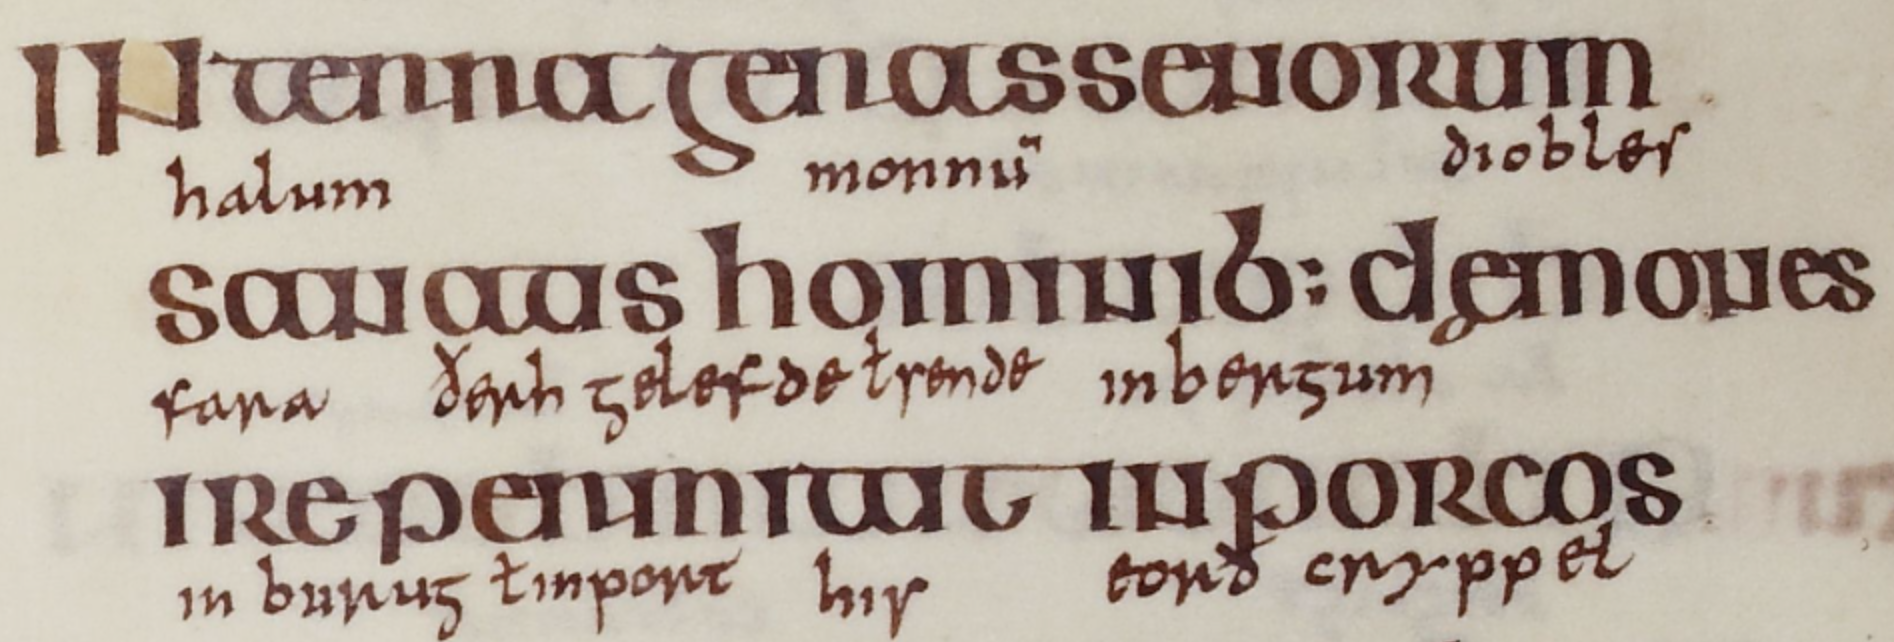
\includegraphics[scale=0.3]{chapters/img/lindisfarne.png}
    \caption{Part of the Lindisfarne Gospels. The larger, blockier text is in \ili{Latin} and dates from around the year 700. Above it, in a smaller hand, a \textsc{gloss} (word-by-word translation) in Northumbrian Old English\il{Old English, Northumbrian} has been added. This dates from the tenth century. Image from\is{manuscripts} \url{http://www.bl.uk/manuscripts/FullDisplay.aspx?ref=Cotton_MS_nero_d_iv}, f. 20v; accessed May 2020.}
    \label{fig:lindisfarne}
\end{figure}

We can be sure that several other languages were spoken in Britain during the period, though. One of these was \ili{Norse} -- the language of settlers from Scandinavia. In addition, Celtic languages were widely spoken throughout the Isles, and large numbers of people must have been bilingual\is{multilingualism} in Brythonic Celtic and Old English. These languages have left their mark on English over the centuries, and as early as Old English we can see their influence in texts. The following two subsections discuss the \ili{Norse} and Celtic contact situations, and we will be returning to the theme of language contact and coexistence throughout the chapter.

\subsection{Scandinavian settlement and rule}\label{OE-Scandinavian}\il{Norse|(}\is{Vikings|(}

According to the \textit{Old English Chronicle}, three ships of \emph{norðmanna} `men of the North' arrived in England in the year 789. They met the reeve, a local official, who tried to make them come quietly to see the king, \emph{þy he nyste hwæt hi wæron} `because he did not know what they were'. This did not end well for the reeve, who was killed. Shortly afterward, in June of 793, the island monastery of Lindisfarne off the north-east coast of England was attacked and looted by ``heathen men'' -- what we now call Vikings. For all intents and purposes, this was the start of the brief but dramatic period of the history of English during which it was shaped by contact with the Norse language.\footnote{Two recent TV series -- \textit{Vikings} (2013--) and \textit{The Last Kingdom} (2015--) -- cover the events of early contact between Norse-speakers and English-speakers. Both aim for entertainment rather than faithfulness, but are a good way to get the gist of the historical events of this period.}

In history books, much is made of the early years of Viking raids on the coasts of Britain. For linguistic purposes, what's really interesting is what happened next: the Chronicle for 876 states that the Scandinavians settled in England, and ``proceeded to plough and support themselves''. This migration\is{migration} continued for at least the next hundred years, and from this point onwards the Scandinavian incomers were a central part of the ethnic and linguistic makeup of Britain itself. Although there is debate about exactly how many settlers from Scandinavia there were (see \citealp{Sawyer1971} for a sceptical view), the consensus today among historians and archaeologists\is{archaeology} is that the scale of settlement was large \citep{Hadley1997,Hadley2009,KershawRoeyrvik2016}, especially in the east and north-east of England. Most of these settlers came from what is now Denmark, though the tenth century also saw settlers from Norway in the north-west of the country.\footnote{Sometimes these later settlers are also referred to as ``Vikings'', but this is misleading: ``viking'', i.e. raiding, was an activity, and it makes little sense to lump all Scandinavian immigrants\is{migration} to Britain together.}

Boundaries between political entities were fluid during the Old English period. Pre-Viking England was a patchworth of small, shifting kingdoms, including Northumbria in the north-east, Mercia in the centre of England, Kent in the south-east, and Wessex in the south. Linguistically and politically, Wessex was the most important of these in the late ninth century, and at this time its ruler Alfred\ia{Alfred (King of Wessex)} reached agreements with the leadership of the Scandinavian incomers through a mixture of military success, diplomacy, and bribes. The Scandinavian king, Guthrum,\ia{Guthrum} converted to Christianity in 878.\is{Christianity}

The language of the Scandinavian settlers, which we've labelled \textsc{Norse}, was a Germanic language closely related to Old English (see \chapref{prehistory} for more on the Germanic family). It's even likely that, with a bit of effort and a sympathetic ear, Norse and Old English were mutually intelligible \citep{Townend2002}. This would have come in handy, as the fate of the settlers and their descendants was inextricably intertwined with that of the Old English speakers: they not only fought but also traded, farmed, ruled, worshipped, and in many cases lived together, depending on the area. The situation was far more nuanced than simply two rival groups: for instance, Alfred's court was visited by a friendly Norwegian, Ohthere\ia{Ohthere} of Hålogaland, who gave him an account of his travels in the far north which still survives in the Old English text \emph{Orosius}.\ia{Orosius, Paulus} Politically, the landscape shifted in the tenth century, and by 1016 the Danish prince \iai{Cnut} was able to claim rule of all of England (advised by a writer and speaker of Old English, the powerful Archbishop Wulfstan of York)\ia{Wulfstan} -- though power returned to Alfred's descendants in the House of Wessex in 1042 after the death of Cnut's sons Harold and Hartha\-cnut. After this, and particularly after the Norman Conquest,\is{Norman Conquest} Norse as a spoken language died out in England, though we don't know exactly when.\footnote{In the Orkney and Shetland Isles off the north coast of Scotland, Norse (known as \textsc{Norn}) survived as late as the eighteenth century \citep{Barnes1998}.}

Other than a handful of inscriptions, we have virtually no evidence for the Norse actually spoken in Great Britain during this period, as it never became a language of writing. However, we can infer a lot about its spoken form from the Old Norse writings of Scandinavia, and from these it becomes very clear that Norse had a huge impact on English, from morphology to syntax to lexicon. We'll look at some examples as we go through.\footnote{For more detail and evaluations of the Norse-English contact situation overall, see \citet{Dance2012}, \citet{Lutz2012}, and \citet{Warner2017}.}\il{Norse|)}\is{Vikings|)}


\begin{peoplebox}{King Alfred}
\ia{Alfred (King of Wessex)|(}
\begin{wrapfigure}{r}{0.35\textwidth}
    \centering
    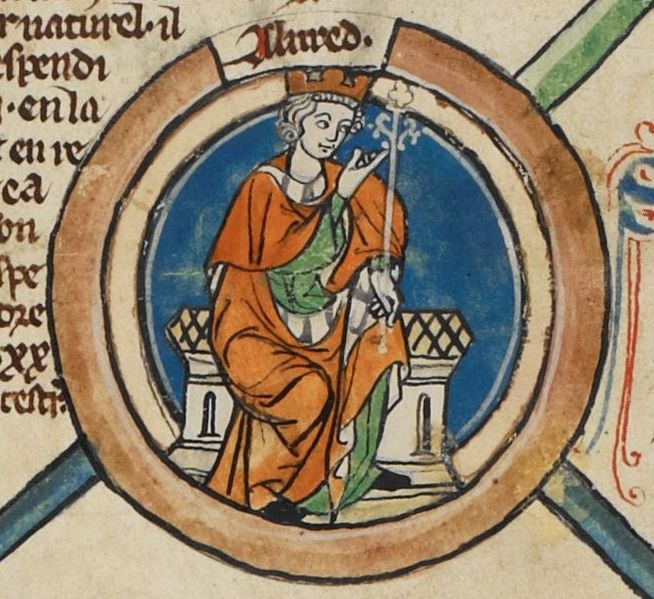
\includegraphics[scale=0.23]{chapters/img/Alfred.jpg}
    \caption{Fourteenth-century manuscript\is{manuscripts} miniature of King Alfred}
    \label{fig:OE_Alfred}
\end{wrapfigure}

Alfred (\emph{Ælfrēd}), King of Wessex from 871 until his death in 899 and later known as ``the Great'', is an important figure for the history of English not just because of his dealings with the Scandinavians. He also played an important role in the establishment of (Old) English as a language of writing, where previously Latin had been dominant. The preface to the Old English translation of Pope Gregory's\ia{Gregory (Pope)} \emph{Pastoral Care}, traditionally attributed to Alfred, writes of Alfred's desire to see more works of learning translated into English, and claims that the standard of learning in England has declined (some things never change). Most of our Old English texts come from Wessex and date to Alfred's reign or later. At one point, Alfred was thought to be personally responsible for writing a wide range of Old English texts, but some scholars nowadays are sceptical about this, suggesting instead that he commissioned and circulated some of these works, and that others had nothing to do with him at all until after his death (see \citealp{Godden2007} vs. \citealp{Bately2009}). In one recent linguistically-informed account \citep[143]{Timofeeva2018},

\begin{quote}
    Alfred's role is seen primarily as that of the social leader whose patronage of a network of Winchester-based scholars gave them the means and stimulus to embark upon a cultural programme that included several extended translations (no matter how many and by whom) and a number of vernacular texts.
\end{quote}

A readable account of King Alfred and Britain during his lifetime can be found in \citet{Adams2017}, and for more detail see the chapters in \citet{DiscenzaSzarmach2015}, which contains a bibliography on the authorship issue.
\end{peoplebox}\ia{Alfred (King of Wessex)|)}


\subsection{Old English and Celtic}\label{OE-Celtic}\il{Celtic, Brythonic|(}

Long before the Scandinavian settlement, Old English in Great Britain coexisted with Celtic languages.

Today's Celtic languages are spoken only on the western side of Great Britain and in Brittany in France. The more northerly Celtic languages -- \ili{Irish} in Ireland, Scottish Gaelic\il{Gaelic, Scottish} in Scotland, and \ili{Manx} on the Isle of Man in the Irish Sea -- are known as the Goidelic languages, and the more southerly -- \ili{Welsh} in Wales, \ili{Cornish} in Cornwall, and \ili{Breton} in Brittany -- are known as Brythonic (or Brittonic).\footnote{Like \ili{Norse} and Old English, the Celtic languages are Indo-European languages (see \chapref{prehistory}). However, the Celtic languages are much more distant relatives, and certainly would not have been mutually intelligible with Old English.} As can be seen in Figure \ref{fig:OE_Celtic}, these languages are not widespread. Almost all the speakers of Celtic languages today are fluent in at least one other language: normally modern English, or modern \ili{French} in the case of \ili{Breton}. For all six languages, active revitalization efforts are ongoing. \ili{Cornish} and \ili{Manx} were even considered extinct for a time in the twentieth century.

\begin{wrapfigure}{r}{0.41\textwidth}
    \centering
    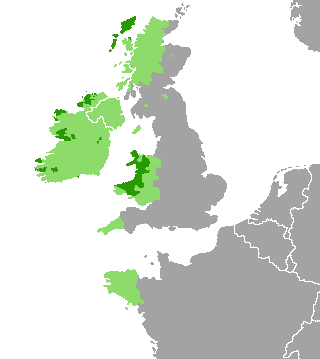
\includegraphics[scale=0.6]{chapters/img/Lenguas_celtas.png}
    \caption{Areas where Celtic languages are spoken today. Dark and light green areas indicate majority and minority usage respectively. (Map by Fobos92, licensed under CC-BY-SA 3.0)}
    \label{fig:OE_Celtic}
\end{wrapfigure}

It wasn't always like this. During the Old English period, in particular, the Celtic languages were much more widely spoken than they are today. Ireland, Scotland and Wales never came under the rule of Old English native speakers, and the same can be said for large parts of what is now England. Devon, in the south-west, was only conquered by Wessex in the early eighth century, and Cornwall not until the very end of the period, in 1086 \citep{Wakelin1975}. Cumbria, in the north-west, was also never firmly under the control of Old English rulers during this period. People in all these areas would have been predominantly Celtic-speaking. And the nature of political control and identity in kingdoms such as Northumbria, Mercia and Wessex was such that we know there must have been a large number of Celtic speakers in these areas too.

Texts and archaeological\is{archaeology} evidence from the early Old English period are fairly sparse and difficult to interpret, so we don't know as much as we'd like about the relationships between Celtic and Old English speakers, and it must have varied from place to place. However, evidence from the Old English lexicon gives us a hint as to the status of Brythonic Celtic speakers in kingdoms like Wessex. The word \emph{wealh}, in particular, could mean `foreigner', `person of Celtic-speaking origin', or `enslaved\is{slavery} person' \citep{Pelteret1995,Lutz2009}; the last of these senses seems to have been limited to the south of England. The word \emph{wīln}, which comes from \emph{wealh-in} (with a feminine suffix),\is{affixes} only ever means `enslaved female'. This lexical evidence suggests that people of Celtic-speaking origin were very often enslaved\is{slavery} in the Old-English-speaking kingdoms. There's also legal\is{legal language} evidence in the form of the laws of King Ine of Wessex, drawn up at the end of the seventh century \citep{Grimmer2007,Woolf2007}. In these documents, the \emph{wergild}\footnote{Money to be paid in compensation for a crime -- in this case, someone's killing.} for a \emph{wilisc mon} (presumably a Celtic speaker) is mentioned explicitly, and contrasted with that of an \emph{englisc mon} (presumably an Old English speaker): a \emph{wilisc mon}\footnote{Directly cognate with Present Day English \textit{Welsh man}.} is worth much less, though there were some \emph{wilisc} landowners. What we can infer from all this evidence is that there were Celtic speakers in the kingdom of Wessex, and probably quite a lot of them, with generally lower social status than speakers of Old English. \citet{Higham1992} suggests that the Old English speakers were in fact only a small, aristocratic minority, with speakers of Celtic making up the majority.

Despite this clear historical evidence for societal multilingualism,\is{multilingualism} the question of Celtic linguistic influence on English has been much more controversial than the question of \ili{Norse} influence. This is partly due to the fact that the historical picture of Celtic-English contact outlined above has only become clear since the 1990s (see \sectref{prehistory-arrival} for more on this), and the details are still a matter of debate. It's partly also due to the relative rarity of the most obvious kind of language contact influence -- lexical borrowings\is{borrowings} (see \sectref{OE-borrowing} later in this chapter). Many instances of potential Celtic influence on English throughout its history have been contested: an example is \emph{DO}-support,\is{\emph{DO}-support} as discussed in \sectref{EModE-do} (see \citealp{vanderAuweraGenee2002}). There are some clear cases, however, even in the Old English period. The best example is probably the uses of the forms of the verb \textit{BE} in Old English, which we'll introduce in \sectref{OE-be}. For overviews of Celtic influence on English see \citet{FilppulaKlemolaPaulasto2008} and \citet{Hickey2012}.\il{Celtic, Brythonic|)}

\subsection{Old English texts}\label{OE-texts}

Nearly a millennium has passed since the Old English period, and the ravages of time have meant that we don't have as many Old English texts as we'd like. We can actually be very specific about this: the Dictionary\is{dictionaries} of Old English \glossterm{gl-corpus}{Corpus},\is{corpora} which contains at least one copy of every known Old English text, comes to just over three million words of Old English.\footnote{See \url{https://tapor.library.utoronto.ca/doecorpus/}.} For comparison, the seven books of the \emph{Harry Potter} series are made up of just over one million words.

The corpus\is{corpora} of Old English texts isn't just very limited -- it's also very skewed. Because literacy\is{literacy} was part and parcel of the Church,\is{Christianity} all the texts we have were produced in a religious context, and most of them have overtly religious themes. Outside religious orders, only a few aristocratic Old English speakers would ever have had access to writing. We don't know who wrote the vast majority of the Old English texts that have come down to us; there are only  handful of exceptions, such as the prolific Abbot \iai{Ælfriċ} of Eynsham and the influential Archbishop \iai{Wulfstan} of York, both of whom were active around the year 1000.

It's certain that, like any living language, Old English as actually spoken exhibited huge amounts of variation geographically, socially and stylistically. But we simply don't have access to most of this variation. Starting with dialects, we can roughly divide Old English texts into four groups:\is{regional variation} West Saxon, Kentish, Mercian, and Northumbrian\il{Old English, Northumbrian}\il{Old English, Kentish}\il{Old English, Mercian}\il{Old English, West Saxon} (the last two are often grouped together as \textsc{Anglian}).\il{Old English, Anglian} However, the emergence of Old English as a written language was linked to the activities of King Alfred of Wessex,\ia{Alfred (King of Wessex)} and so it's not a surprise that almost all of our Old English texts are written in the West Saxon\il{Old English, West Saxon} dialect.\footnote{Or at least the versions that have come down to us are in West Saxon. For some texts, like \textit{Beowulf}, there is evidence to suggest that they were originally composed in a different dialect and only translated later into West Saxon.} And, when we can localize the texts at all, we find that they come from a small number of scribal\is{scribes} centres (see Figure \ref{fig:OE_locations} for some of the most important).

\begin{figure}[!ht]
     \centering
     \begin{tikzpicture}
        \node[align=center] (map) at (6,4)
        {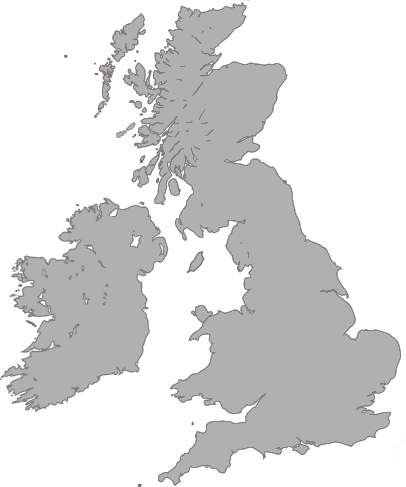
\includegraphics[width=.6\textwidth]{chapters/img/blank-uk.png}};
        \filldraw[fill=lsLightGreen,draw=black] (0,0) rectangle (4.5,2.5);
        \node[align=center] (WestSaxon) at (2.25,1.25) {\textbf{West Saxon}\\Old English Chronicle\\(Parker MS)\\Orosius (Lauderdale MS)};
        \filldraw[fill=lsMidBlue,draw=black] (0.3,4.8) rectangle (3.8,7.2);
        \node[align=center] (Mercian) at (2.05,6) {\textbf{Mercian}\\Vespasian Psalter\\Corpus Glossary\\Épinal Glossary};
        \filldraw[fill=lsLightWine,draw=black] (9,2.8) rectangle (12,4.3);
        \node[align=center] (Kentish) at (10.5,3.55) {\textbf{Kentish}\\Kentish Glosses};
        \filldraw[fill=lsYellow,draw=black] (8,6) rectangle (11.5,8);
        \node[align=center] (Northumbrian) at (9.75,7) {\textbf{Northumbrian}\\Lindisfarne Gospels\\Durham Ritual};
        \draw[->] (10.5,2.8) -- (9.3,0.77);%Kentish
        \node[align=center] (Canterbury) at (10.25,0.77) {\footnotesize{Canterbury}};
        \draw[->] (9.75,6) -- (7.65,4.3);%Northumbrian
        \node[align=center] (CLS1) at (7.2,4.1) {\footnotesize{Chester-}};
        \node[align=center] (CLS2) at (7.5,3.8) {\footnotesize{le-Street}};
        \draw[->] (4.5,1.25) -- (7.8,0.5);%WS
        \node[align=center] (Winchester) at (7.8,-0.1) {\footnotesize{Winchester}};
        \draw[->] (3.5,6.3) -- (7.4,2.1);%Mercian
        \node[align=center] (Lichfield) at (7.4,1.9) {\footnotesize{Lichfield}};
     \end{tikzpicture}
     \caption{Some key scribal\is{scribes} centres during the Old English\il{Old English, Northumbrian}\il{Old English, Kentish}\il{Old English, Mercian}\il{Old English, West Saxon}\ia{Orosius, Paulus} period}
     \label{fig:OE_locations}
\end{figure}

We have enough Old English material to see it changing over time, though. Texts from the early part of the period -- before Alfred's\ia{Alfred (King of Wessex)} reign in the late ninth century -- are few and far between, but some have survived, like the seventh-century \emph{\iai{Cædmon}'s Hymn} and the seventh-eighth-century Épinal and Erfurt glossaries. Texts from before 900, including those from Alfred's\ia{Alfred (King of Wessex)} reign, are known as \textsc{Early Old English} texts: these include many translations from \ili{Latin}, including \iai{Boethius}'s \emph{Consolation of Philosophy} and \iai{Bede}'s \emph{Ecclesiastical History of the English People}. Old English from between 900 and 1150 is labelled \textsc{Classical} and is dominated by the works of \iai{Wulfstan} and especially \iai{Ælfriċ}. From this period we have many sermons and stories of the lives of saints, but also scientific texts\is{scientific language} such as \iai{Byrhtferth}'s \emph{Enchiridion} (`manual') and medical handbooks like the \emph{Herbarium}. And from across the whole Old English period we have legal documents,\is{legal language} as well as the famous \textit{Old English Chronicle}, a year-by-year retelling of historical events that survives in several manuscripts.\is{manuscripts}

The nature of the texts that survive is heavily determined by who wielded (political and religious) power. The majority of our texts are West Saxon\il{Old English, West Saxon} and date from the late ninth century onwards, due to the preeminence of the kingdom of Wessex during this period. By contrast, the earlier texts have a strong Northumbrian\il{Old English, Northumbrian} or Mercian\il{Old English, Mercian} flavour, since the kingdoms of Northumbria and Mercia had their heydays in the seventh and eighth century respectively.\footnote{If you're interested in the thorny issues of disentangling dialectal and scribal\is{scribes} from diachronic variation in Old English texts, we recommend you take a look at \citet{Hogg1988}, ``On the impossibility of Old English dialectology''.} We'll return to some of the main differences between early and late Old English in \sectref{OE-morphology} and \sectref{OE-syntax}.


\begin{peoplebox}{Women writers in early England}
\begin{wrapfigure}{l}{0.35\textwidth}
    \centering
    \includegraphics[scale=0.055]{chapters/img/Of_Runes_and_Saints.jpg}
    \caption{Hild of Whitby on a church banner. Note the runic\is{runes} letters! (Photo by Jonund, licensed under CC-BY-SA 2.0)}
    \label{fig:OE_Hild}
\end{wrapfigure}

All of the named writers of Old English that we know of are men. This makes it rather difficult for us to know how human gender may or may not have been expressed through language at the time.\is{gender studies} The earliest named women writers whose work has been passed down to us are only from the Middle English period (see \sectref{ME-text-transmission}). That doesn't mean, however, that women weren't active as writers and patrons of writing during the Old English period. Religious\is{Christianity} houses in medieval England could be male-only, female-only and mixed, and abbesses like \iai{Hild of Whitby} (614--680; patron of the poet\is{poetry} \iai{Cædmon}) and \iai{Æthelthryth of Ely} (c. 636--679) wielded a great deal of spiritual, political and economic power. The texts known to have been written by women from this period are in \ili{Latin} rather than Old English, but some Old English texts such as \textit{Wulf \& Eadwacer} and \textit{The Wife's Lament} are female-voiced. \citet[58--68]{Watt2019} suggests that the Old English fragments of the \textit{Life of St Mildrith} were written by a woman, especially given the text's focus on female authority, power, and heritage.\footnote{For more on women and writing in early medieval England see \citet{LeesOvering2001}, \citet{Watt2019}, and\is{manuscripts} \url{https://blogs.bl.uk/digitisedmanuscripts/2018/12/women-and-books-in-anglo-saxon-kingdoms.html}.}
\end{peoplebox}


\noindent Finally, no section on Old English texts would be complete without mentioning the period's poetry,\is{poetry} often seen as the best reason to learn to read Old English from a literary perspective. Most surviving Old English poetry is contained within just four manuscripts:\is{manuscripts} the Junius manuscript, the Exeter Book, the Vercelli Book, and the Nowell Codex. In the poetry we can find a mix of Christian\is{Christianity} and pre-Christian influences. Old English poetry is alliterative\is{alliteration} rather than rhyming (see \sectref{prehistory-stress} in the next chapter), and deals with a variety of themes. The most famous is \emph{Beowulf}, an epic poem dealing with the eponymous hero's journey from wandering warrior to king and the monsters and challenges he faces along the way.\is{poetry}

\section{Sounds}\label{OE-phonology}

We've come a long way from Modern English, so at this point we should stop and give an overview of the whole sound system of Old English and how it relates to spelling.\is{orthography|(} Table \ref{tab:OE-vowels} presents the vowels\is{vowels} of Old English, and Table \ref{tab:OE-consonants} presents the consonants.\is{consonants}

\begin{table}
    \caption{Old English vowel phonemes and corresponding graphemes}\label{tab:OE-vowels}
  \begin{tabularx}{\textwidth}{XXXl}
\lsptoprule
 ~ & Front unrounded & Front rounded & Back \\
    \midrule
    high & /i, iː/ $\leftrightarrow$ <i> & /y, yː/ $\leftrightarrow$ <y> & /u, uː/ $\leftrightarrow$ <u>\\
    mid & /e, eː/ $\leftrightarrow$ <e> & /ø, øː/ $\leftrightarrow$ <oe> & /o, oː/ $\leftrightarrow$ <o>\\
    low & /æ, æː/ $\leftrightarrow$ <æ> & ~ & /ɑ, ɑː/ $\leftrightarrow$ <a>\\
    \lspbottomrule
  \end{tabularx}
\end{table}

\noindent So far, so straightforward. Old English, like Middle English (see \sectref{ME-lengthening}),\is{vowel lengthening} had both long and short vowel phonemes.\is{vowels} This distinction wasn't represented in writing, though. Sometimes, in modern editions of Old English texts, the editors mark length using a \emph{macron} above the vowel, as in \emph{Ælfrēd}, with <ē>, for the name of the king.\ia{Alfred (King of Wessex)} It's important to note that this macron was never found in manuscripts\is{manuscripts} -- it's a modern addition intended to make life easier for readers.\footnote{We do find the macron in Old English manuscripts, but not to distinguish vowel length.}

We find one grapheme used to represent a sound in the Old English vowel system that we don't see at any other stage of the language: the grapheme <æ>, called \emph{ash}.\is{ash} This is known as a \textsc{ligature}\is{ligature} /ˈlɪɡətʃə/ or \textsc{ligated digraph} /ˈlaɪɡeɪtɪd ˈdaɪɡrɑːf/, and, in simpler words, consists of two characters squished together -- in this case <a> and <e>. It has its own phonemic value, though, which is always /æ/ or /æː/.\is{vowels}

Old English also has diphthongs. Originally, there were eight of these, four long, four short: 

\begin{itemize}
    \item /iu, iːu/ $\leftrightarrow$ <io>
    \item /iy, iːy/ $\leftrightarrow$ <ie>
    \item /eo, eːo/ $\leftrightarrow$ <eo>
    \item /æɑ, æːɑ/ $\leftrightarrow$ <ea>
\end{itemize}

\noindent As can be expected for any period of the language, there is some variation in the vowel system over time in Old English as well. The mid front rounded phonemes /ø/ and /øː/, written as <oe>, are only found in early Old English texts. Later on, they become unrounded\is{unrounding} and merge\is{merger} with /e/ and /eː/. Similarly, half of the diphthongs are lost during the period. By the time of Classical West Saxon,\il{Old English, West Saxon} /iu/ and /iːu/ have merged with /eo/ and /eːo/ respectively, and /iy/ and /iːy/ have merged\is{merger} with /y/ and /yː/. In later Old English texts we also find a very narrow range of vowels in unstressed syllables.\is{vowel reduction} We'll come back to this in \sectref{OE-case-loss}, because it's relevant to morphological changes in the language as well.\is{vowels}


\begin{table}
\small
    \caption{Old English consonant phonemes and graphemes}\is{consonants|(}\label{tab:OE-consonants}
  \begin{tabularx}{\textwidth}{p{1.4cm}p{2cm}QQp{1.2cm}@{}}
\lsptoprule
 ~ & labial & coronal & palatal & velar \\
    \midrule
    voiceless stops & {/p, pː/ $\leftrightarrow$ \newline<p, pp>} & /t, tː/ $\leftrightarrow$ <t, tt> & ~ & {/k, kː/ $\leftrightarrow$ \newline<k, kk>}\\
    \midrule
    voiced stops & {/b, bː/ $\leftrightarrow$ \newline<b, bb>} & /d, dː/ $\leftrightarrow$ <d, dd> & ~ & {/g, gː/ $\leftrightarrow$ \newline<g, gg>}\\
    \midrule
    fricatives & {/f, fː/ $\leftrightarrow$ \newline<f, ff>} & \mbox{/θ, θː/ $\leftrightarrow$ <þ/ð, þþ/ðð>} \newline/s, sː/ $\leftrightarrow$ <s, ss> & {/ʃ, ʃː/ $\leftrightarrow$ <sc>} & {/x, xː/ $\leftrightarrow$ \newline<h, hh>}\\
    \midrule
    voiceless affricates & ~ & ~ & {/tʃ, tʃː/ $\leftrightarrow$ \newline<c, cc>} & ~\\
    \midrule
    voiced affricates & ~ & ~ & {/dʒ, dʒː/ $\leftrightarrow$ \newline<cg or gg>} & ~\\
    \midrule
    nasals & {/m, mː/ $\leftrightarrow$ \newline<m, mm>} & {/n, nː/ $\leftrightarrow$ <n, nn>} & ~ & ~\\
    \midrule
    liquids & ~ & {/l, lː/ $\leftrightarrow$ <l, ll> \newline /r, rː/ $\leftrightarrow$ <r, rr>} & ~ & ~\\
    \midrule
    glides & {/w, wː/ $\leftrightarrow$ \newline<uu or ƿ, ƿƿ>\footnote{The grapheme <w> is found in almost all modern editions of Old English texts, but not in the manuscripts.\is{manuscripts} Old English scribes\is{scribes} either used <uu>, i.e. a literal ``double u'', or the character <ƿ>\is{wynn} (``wynn''), originally from the runic\is{runes} alphabet (see \sectref{prehistory-runes}).}} & ~ & \mbox{/j, jː/ $\leftrightarrow$ \newline <g/i, gi/ii>} & ~\\
    \lspbottomrule
\end{tabularx}
\end{table}

\noindent Like the vowels,\is{vowels} Old English consonants come in both long and short versions, and the length distinction is phonemic. Long consonants -- also known as \glossterm{gl-geminate}{geminates}\is{geminates} -- are usually represented in the manuscripts\is{manuscripts} by doubling: /bː/, for example, is written as <bb>. These length distinctions could be rather important. Compare for instance \textit{cwelan} /kwelɑn/ `to die' and \textit{cwellan} /kwelːɑn/ `to kill' (or to cause someone to die).

One thing worth noting about Old English, in contrast to Middle English and all subsequent stages, is that there is no \glossterm{gl-phoneme}{phonemic} voicing contrast in fricatives.\is{voicing allophony} Instead, fricatives had both voiced and voiceless \glossterm{gl-allophone}{allophones}. The voiced allophone (e.g. [v] for the phoneme /f/) was found when the fricative is between two voiced sounds, for instance between vowels.\is{vowels}\footnote{But also nasals (/m/, /n/) liquids (/r/, /l/),\is{/r/} approximants (/w/, /j/), and voiced plosives (e.g. /b/).} Otherwise, the voiceless allophone was found. Thus, Old English \textit{wulf} would be pronounced as [wulf], but the plural\is{plurals} \textit{wulfas} as [wulvas]. As we can see, this allophonic difference isn't represented in the spelling, though. The development of a \emph{phonemic} voicing contrast in Middle English and beyond is probably due to contact influence from languages which did possess this contrast. \citet{Laker2009} argues that contact with Brythonic Celtic\il{Celtic, Brythonic} is responsible, and in response \citet{Minkova2011} defends the more conventional view that the change is due to the large number of lexical borrowings\is{borrowings} from \ili{French}. Once the voiced allophones had become phonemes, however, they were often represented as such in the spelling as\is{voicing allophony} well.\footnote{With the exception of the dental fricatives /θ/ and /ð/, which -- as we have seen -- were spelt with either <þ> or <ð> irrespective of the phonetic or phonological status of the phone, and in Present Day English are both spelt with <th>} This gives us the following Present Day English phonological irregularities,\is{irregularities} which are also represented as irregular in the spelling in case of /f/ and /v/: \textit{calf} $\sim$ \textit{calves}, \textit{dwarf} $\sim$ \textit{dwarves}, \textit{hoof} $\sim$ \textit{hooves}, \textit{knife} $\sim$ \textit{knives}, \textit{leaf} $\sim$ \textit{leaves}, \textit{life} $\sim$ \textit{lives}, \textit{wife} $\sim$ \textit{wives}, \textit{house} $\sim$ \textit{houses},\footnote{Though the latter tends to be pronounced with a voiceless fricative in American English.} \textit{oath} $\sim$ \textit{oaths}, \textit{path} $\sim$ \textit{paths}; \textit{breath} $\sim$ \textit{to breathe}, \textit{grief} $\sim$ \textit{to grieve}, \textit{teeth} $\sim$ \textit{to teethe}, and \textit{wreath} $\sim$ \textit{to wreathe}.


\begin{sourcebox}{Thorn and eth}
We met the letter \glossterm{gl-thorn}{thorn}\is{thorn}\is{eth} <þ> in \sectref{ME-graphical}. In Old English, as in Middle English, it's used for both the voiced dental fricative [ð] and the voiceless dental fricative [θ]. As we've noted, these were \glossterm{gl-allophone}{allophones} of a single fricative \glossterm{gl-phoneme}{phoneme}, since fricative voicing was not distinctive in Old English. Another grapheme used for the same phoneme was <ð>, \textsc{eth}. There isn't any consistent difference between <þ> and <ð>: they're used variably to represent the same phoneme\is{voicing allophony} (remember, Old English wasn't \glossterm{gl-standardization}{standardized}\is{standardization} like today's English).\footnote{It has been proposed in the literature that West Saxon\il{Old English, West Saxon} was standardized to some extent; for a sceptical evaluation see \citet{Hogg2006}.} Historically, thorn comes from the runic\is{runes} alphabet (see \sectref{prehistory-runes}), while eth is simply what it looks like: a \ili{Latin} <d> with a bar through it. \citet{DroutChauvet2015} suggest that subtle quantitative differences in the use of <þ> and <ð> can be used to investigate the history and authorship of Old English texts.\is{orthography|)}\is{consonants|)}
\end{sourcebox}


\noindent With this background in mind, we can now turn to two phonological processes that characterize Old English: palatalization (\sectref{OE-palatalization})\is{palatalization} and \emph{i}-umlaut (\sectref{OE-umlaut}).\is{umlaut}

\subsection{Palatalization}\label{OE-palatalization}\is{palatalization|(}
Palatalization\is{consonants|(} is a process which lies behind Present Day English alternations like these:

\begin{itemize}
\item \textit{batch} $\sim$ \textit{to bake}, \textit{bench} $\sim$ \textit{bank}\footnote{In the meaning of `a long, high mound with steeply sloping sides' (OED; 2020, \glossterm{gl-sv}{s.v.} bank, n.1.).}, \textit{to beseech} $\sim$ \textit{to seek}, \textit{birch} $\sim$ \textit{birk}, \textit{chary} $\sim$ \textit{care}, \textit{-chester} $\sim$ \textit{-caster}, \textit{to chill} $\sim$ \textit{cold}, \textit{church} $\sim$ \textit{kirk}, \textit{ditch} $\sim$ \textit{dyke}, \textit{drench} $\sim$ \textit{to drink}, \textit{match}\footnote{As in `a couple' or `a pair', not the short pieces of wood used to light a fire.} $\sim$ \textit{to make}, \textit{milch} $\sim$ \textit{milk}, \textit{stench} $\sim$ \textit{to stink}, \textit{stitch} $\sim$ \textit{stick}, \textit{watch} $\sim$ \textit{wake}, and \textit{-wich} $\sim$ \textit{-wick} (as in the place names \textit{Norwich} vs. \textit{Warwick})
\item \textit{yard} $\sim$ \textit{garden}, \textit{yarn}\footnote{A spun fibre.} $\sim$ \textit{garn}\footnote{A variant of \textit{yarn} attested in the north of Britain\is{regional variation} (OED; 2020, \glossterm{gl-sv}{s.v.} garn, n.).}, \textit{yellow} $\sim$ \textit{golden}, and \textit{to yearn} $\sim$ \textit{to green}\footnote{This word has nothing to do with the colour here: it's a Scottish\il{English, Scottish} word meaning `to yearn, desire' (OED; 2020, \glossterm{gl-sv}{s.v.} green, v.2).}, and \textit{to yell} $\sim$ \textit{nightingale} (the \textit{gale} part)
\item \textit{dish} $\sim$ \textit{disk}, \textit{fish} $\sim$ \textit{piscatorial}, \textit{mesh} $\sim$ \textit{mask}, \textit{shatter} $\sim$ \textit{scatter}, \textit{shave} $\sim$ \textit{scab}, \textit{shell} $\sim$ \textit{scale}, \textit{ship} $\sim$ \textit{skipper}, \textit{shrift} $\sim$ \textit{script}, \textit{shirt} $\sim$ \textit{skirt}, and \textit{shuffle} $\sim$ \textit{scuffle}
\end{itemize}

\noindent It is a process whereby a consonant with a non-palatal place of articulation becomes palatal. Thus, what used to be /k/ (a velar consonant) became /tʃ/ (a palatal one), /g/ became /j/, and /sk/ became /ʃ/, prior to the time from which we have the earliest written records of Old English. But hmmmm, hang on, if that was the case, how come we've still got the pairs such as those mentioned above in Present Day English? There are two reasons for this. 

First, in case of /k/ > /tʃ/ and /g/ > /j/, palatalization only happened when a certain group of vowels\is{vowels} combined with /k/ and /g/. Thus, Present Day English \textit{chill} /tʃɪl/ comes from Old English \textit{ċele} and Present Day English \textit{cold} /kəʊɫd/ comes from Old English \textit{cald}; the surrounding vowels are different, and only some vowels conditioned palatalization. It is not unreasonable to assume that the palatalization of /sk/ to /ʃ/ was initially also limited to certain vowel contexts.\footnote{Palatalization is likely to start in the context of front vowels,\is{vowels} such as /i/ and /e/, and has occurred in the history of many languages. The reason for this probably lies in coarticulatory effects and systematic patterns of misperception by listeners (see \citealp{Ohala1989}). In pre-Old English specifically, consonants underwent palatalization when immediately followed by a front unrounded vowel or by a palatal glide, or when word-final after a front unrounded vowel.} However, by the end of Old English, /sk/ had palatalized to /ʃ/ irrespective of which vowel preceded or followed. So it is only the /k/ $\sim$ /tʃ/ alternations that can be explained by the vocalic\is{vowels} environment of the words involved. 

The second explanation is related to chronology. At some point, /sk/ started changing into /ʃ/. This took a while, but, eventually, this process stopped being active. There were no more /sk/s left to be affected by palatalization. That is, until speakers of English came into contact with other languages, and languages which had not undergone the same process of palatalization and therefore had /sk/ and/or /k/ in various vowel\is{vowels} contexts. Contact with languages such as \ili{Norse}, \ili{Latin}, and \ili{French} can therefore also explain the alternations we see above: words with /sk/ and /k/ that were borrowed\is{borrowings} into English after palatalization stopped being an active process, i.e. during or after the period of attested Old English, retained their non-palatalized consonants. Is it a coincidence that \textit{kirk}, related to \textit{church} (from Old English \emph{ċirice}), is typically used in Scotland,\il{English, Scottish} considering that the presence of Scandinavian speakers was skewed towards the north and east of the island?\is{regional variation}

The word pairs provided in the bullet points above are therefore due to a combination of these two reasons. For instance, \textit{fish} and \textit{shatter} show Old English palatalization, while the non-palatalized counterparts, \textit{piscatorial} and \textit{scatter}, are loans\is{borrowings} from Latin and Old Norse, which had not undergone palatalization. On the other hand, \textit{to yell} underwent palatalization due to the following non-low front vowel, while \textit{nightingale} did not because the following vowel\is{vowels} was too low and back for palatalization to happen.

The lack of seemingly expected palatalization, as in e.g. \textit{disk} and \textit{skirt}, may however not be only due to language contact and within-dialectal vowel\is{vowels} environment. An outcome of this type may also have to do with regional differences\is{regional variation} present in Old English which affected the types of vowels that preceded and/or followed /g/, /k/, or /sk/. What this means is that where one dialect may have had a /g/, /k/, and /sk/ followed by an /e/, /ɪ/ or /j/, another dialect may have had the same consonant followed by an /ɑ/, which means that that the words in the dialect of the latter group wouldn't have undergone the process of palatalization. Because settlement of Old Norse speakers geographically heavily overlaps with these dialects, it can be quite tricky to be sure whether a non-palatalized consonant (e.g. \textit{dike} vs \textit{ditch}) is due to regional variation,\is{regional variation} language contact with Old Norse, or indeed a mixture of the two. Linguists have been arguing about such matters quite passionately, and gathering and assessing the evidence can be a fairly tricky business. A case in point is indeed for instance the word \textit{dike} (see \citealp{Ramisch1997}, who argues these variants are more likely due to dialectal variation rather than language contact with Old Norse).

Palatalization has an awkward effect on how a speaker of Present Day English should make sense of some of the Old English spellings, as palatal phonemes do not usually have their own corresponding grapheme in Old English manuscripts.\is{orthography}\is{manuscripts} The letter <c> can thus represent either /tʃ/ or /k/, and similarly the letter <g> can represent either /j/ or /g/. If you know the conditions under which palatalization took place in pre-Old English, you can figure out which phoneme to pronounce when you read <c> or <g>. But this is hard work requiring knowledge reaching far beyond even that of Old English, and to make it easier for the modern reader, many editors of Old English texts have adopted the convention of \glossterm{gl-overdotting}{overdotting}, representing the palatal sounds /ʃ/, /tʃ/, /dʒ/, and /j/ as <sċ>, <ċ>, <ċġ>, and <ġ> respectively. For example, the Old English word for \textit{yellow} is written with an overdotted g: \emph{ġeolu}. This makes life easier for the reader, but it's important to remember that overdotting, like the macron that editors use for long vowels,\is{vowels} was not present in Old English\is{manuscripts} manuscripts.\footnote{At least not for this purpose.}

If palatalization seems a little bit alien to you, know that palatalization is happening (yes, again!) in Present Day English as well, right under our noses. Think for instance of pronunciations such as \textit{wantcha} and \textit{gotcha}, or even \textit{wouldja}, for \textit{want you}, \textit{got you}, and \textit{would you}, whereby the following palatal sound, /j/, affects the preceding consonant, /t/ and /d/ in our cases, making them into /tʃ/ and /dʒ/, respectively. (So in other words, /t/ and /d/ have palatal versions today in some contexts as well!)\is{palatalization|)}


\begin{soundbox}{How were /r/s pronounced in Old English?}
\is{/r/}
You might be wondering, as many people studying Old English do, just how exactly the <r> was pronounced. Was it a trill ([r]), was it an alveolar approximant ([ɹ]), or even a retroflex approximant ([ɻ]), or, yes, even a uvular voiced fricative ([ʁ])? Most Present Day English dialects have an alveolar approximant ([ɹ]) or a retroflex approximant ([ɻ]). So perhaps one could assume that this must have been the realization in Old English too? Good thinking, but Present Day English has more to offer than just these two variants: a stereotypical feature of Scottish English\il{English, Scottish} is the trilled [r] and a now moribund feature of Northumbrian English\il{English, Northern England} is the so-called Northumbrian burr, which refers to a uvular fricative [ʁ] \citep[368--370]{Wells1982b}.\is{regional variation} We can't rule out that these lesser-represented Present Day English variants used to be more widespread in the past stages of the language. As the next step, we could also look to other Germanic languages spoken today, but once we start looking closely enough, we will find a wonderfully rich well of variation as well. If we take \ili{Dutch}, for instance, \citet[29]{Sebregts2014} mentions 16 variants of /r/, and that's still not quite the full picture. To cut a long story short, then, it's very likely that regionally conditioned variation\is{regional variation} existed in Old English /r/, and the take-home message for you is not to worry too much about how you pronounce /r/s when reciting Old English poetry\is{poetry} (or prose!), as long as you do pronounce an /r/ consonant of some sort.\is{consonants|)}
\end{soundbox}


\subsection{\emph{i}-umlaut}\label{OE-umlaut}\is{umlaut|(}
In\is{vowels|(} Present Day English, we find words which look like they must be related in one way or other, and which show vowel differences, as in 

\begin{itemize}
\item \textit{brother} $\sim$ \textit{brethren}, \textit{foot} $\sim$ \textit{feet}, \textit{goose} $\sim$ \textit{geese}, \textit{tooth} $\sim$ \textit{teeth}, \textit{man} $\sim$ \textit{men}, \textit{woman} $\sim$ \textit{women}, \textit{louse} $\sim$ \textit{lice}, and \textit{mouse} $\sim$ \textit{mice}
\item \textit{blood} $\sim$ \textit{to bleed}, \textit{food} $\sim$ \textit{to feed}, \textit{sale} $\sim$ \textit{to sell}, \textit{tale} $\sim$ \textit{to tell}, and \textit{tooth} $\sim$ \textit{to teethe}
\item \textit{broad} $\sim$ \textit{breadth}, \textit{foul} $\sim$ \textit{filth},  \textit{long} $\sim$ \textit{length}, and \textit{strong} $\sim$ \textit{strength}
\item \textit{old} $\sim$ \textit{elder} (and \textit{eldest})
\item \textit{to bring} $\sim$ \textit{brought}, \textit{to buy} $\sim$ \textit{bought}, \textit{to seek} $\sim$ \textit{sought}, \textit{to sell} $\sim$ \textit{sold}, \textit{to teach} $\sim$ \textit{taught}, \textit{to tell} $\sim$ \textit{told}, \textit{to think} $\sim$ \textit{thought}, and \textit{to work} $\sim$ \textit{wrought}\footnote{The form \textit{wrought}, rather than \textit{worked}, is now archaic and/or used in fairly specific contexts.}
\item \textit{full} $\sim$ \textit{to fill}
\item \textit{fox} $\sim$ \textit{vixen}, \textit{cat} and \textit{kitten}, and \textit{theft} $\sim$ \textit{thief}
\end{itemize}

\noindent In these examples, we see primarily the following spelling alternations:\is{orthography}

\begin{itemize}
\item <o> $\sim$ <e>, <oo> $\sim$ <ee>, <oa> $\sim$ <ea>
\item <a> $\sim$ <e>
\item <u>, <ou> $\sim$ <i>
\end{itemize}

\noindent As we saw in Chapters \ref{EModE} and \ref{ME}, these letters\is{orthography} reflect the pre-Great Vowel Shift\is{Great Vowel Shift} pronunciations:

\begin{itemize}
\item <goose> /goːs/ $\sim$ <geese> /geːs/
\item <man> /mɑn/ $\sim$ <men> /men/
\item <mouse> /muːs/ $\sim$ <mice> /miːs/
\end{itemize}

\noindent So this corresponds to the pairing of the following sounds for most of the examples given above:\footnote{We ignore the effects of umlaut on diphthongs for simplicity's sake.}

\begin{itemize}
\item /o/, /oː/ $\sim$ /e/, /eː/
\item /ɑ/ $\sim$ /e/
\item /uː/ $\sim$ /iː/
\end{itemize}

\noindent These vowel alternations serve the following functions in the Present Day English pairs mentioned above: plural\is{plurals} formation (\textit{mouse} $\sim$ \textit{mice}), deadjectival noun formation (\textit{strong} $\sim$ \textit{strength}), deadjectival verb formation (\textit{full} $\sim$ \textit{to fill}), the comparative (and the superlative; e.g. \textit{old} $\sim$ \textit{elder} $\sim$ \textit{eldest}), verb-verb word-formation processes (\textit{to fall} $\sim$ \textit{to fell}), and ultimately derivational processes related to noun-noun pairs (\textit{fox} $\sim$ \textit{vixen}). In Old English, these alternations served these functions too, but we find two important differences. First of all, these vowel patterns were not limited to just a handful of words, as in Present Day English, where non-native speakers have to rather painfully memorize these. Secondly, these various functions were not the only functions these vowel alternations had. And we should also add one more difference: this process was not limited to the vowel pairs provided above. 

But what is this vowel alternation process that we've been discussing, and how did it come about? The process involved in this mystery is the so-called \textsc{umlaut}, also known as \emph{i}-umlaut, mutation, and \emph{i}-mutation. It is a type of vowel assimilation, whereby one vowel becomes more like another. 

More specifically, umlaut is a phonological process that happened prior to Old English (see more in \chapref{prehistory}). If a word had, for instance, two syllables, and the second one contained either /i/ or /j/, the vowel in the first syllable became more like this /i/ or /j/. In other words, it assimilated. It is useful here to remind ourselves of the vowel space, as shown in Figure \ref{fig:umlaut}. When looking at the figure first, ignore the red parts. Different vowels have different positions in the vowel space -- they differ in terms of height and backness/frontness.

\begin{figure}
%     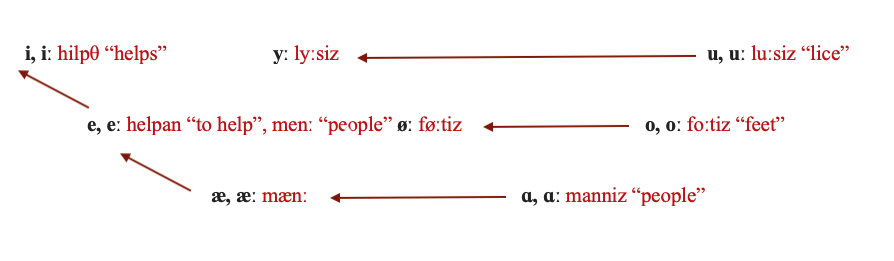
\includegraphics[scale=0.4]{chapters/img/umlaut.png}
    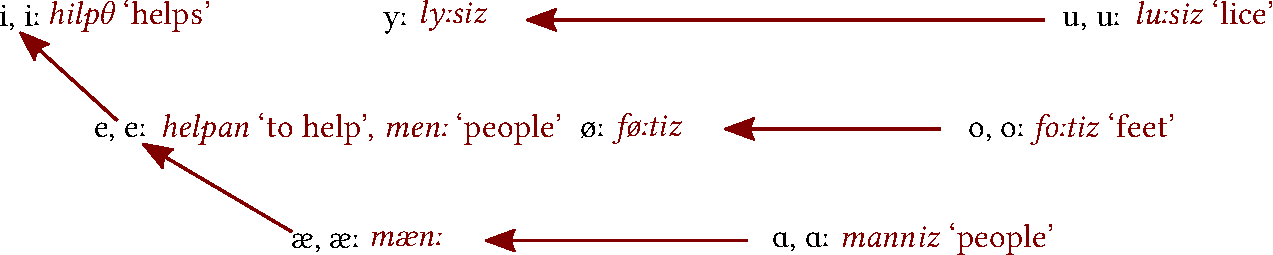
\includegraphics[width=\textwidth]{chapters/img/umlaut_mod.pdf}
    \caption{Vowel-specific changes under the process of \emph{i}-umlaut}
    \label{fig:umlaut}
\end{figure}

When umlaut happened, imagine each of these vowels moving closer to an /i/ (or a /j/, which we can think of as a very short, consonantal\is{consonants} version of /i/).\footnote{Try saying /j/ and holding the consonant for a while. What happens when you do so?}

Thus, the following Old English vowels changed as follows under the influence of umlaut:
\begin{itemize}
\item /u/, /uː/ > [y], [yː]; they fronted, remaining round; as in \textit{mus} `mouse' $\sim$ \textit{mys} `mice', ultimately \textit{mis}
\item /o/, /oː/ > /ø/, /øː/; they fronted, remaining round; as in \textit{dom} `doom' $\sim$ \textit{doeman}, ultimately \textit{deman} `to deem, judge'
\item /e/, /eː/ > /i/, /iː/; they were raised and just a little bit fronted; as in \textit{helpan} `to help' $\sim$ \textit{hilpð} `he/she/it helps'
\item /ɑ/, /ɑː/ > /æ/, /æː/; as in \textit{mann} `man' $\sim$ \textit{mænn} `men', and ultimately \textit{menn}\footnote{Long /ɑː/ and /eː/ apparently did not always undergo umlaut, and the development of /ɑː/ differed in different dialects \citep[159--160]{Minkova2014}.}
\end{itemize}

\noindent [øː] is a front rounded vowel, which unrounded\is{unrounding} fairly early on to [eː], so we often find it spelt in a way suggestive of [eː] (e.g. <e>) rather than [øː] (e.g. <oe>) in Old English texts. Towards the end of the Old English period, the same started happening to [yː], which ultimately unrounded\is{unrounding} to [iː]. These sounds are phonemic in Old English, but were allophonic prior to Old English. Most of the forms created by \emph{i}-umlaut eventually died out -- the plural\is{plurals} of \emph{cow} is no longer \emph{kine}, for example, and the plural of \emph{book} is no longer \emph{beech} -- but some frequent\is{frequency} ones, including those listed above, have survived and any teacher has to deal with them.

As mentioned, umlaut is what's known as a \textsc{conditioned} sound change: it only affected vowels when the following syllable contained an /i/ or a /j/. What's tricky about umlaut is that this /i/ or /j/ in the subsequent syllable was mostly lost, like many of the vowels in unstressed syllables\is{vowel reduction} -- after umlaut had taken place, but before the Old English texts that have come down to us. Thus there's nothing in the word \emph{men}, for instance, to indicate that there used to be an extra syllable on the end containing an /i/. In many cases, umlaut itself is the only evidence that this /i/ was ever there in the first place.

And if you're wondering about whether these alternations are also due to umlaut:

\begin{itemize}
    \item \textit{sing} $\sim$ \textit{sang} $\sim$ \textit{sung}
    \item \textit{ride} $\sim$ \textit{road}
\end{itemize}

\noindent then let's just say right now that these can be explained through a different process, which you can read more about in \sectref{prehistory-strong} in the next chapter.\is{umlaut|)}


\begin{soundbox}{The case of \textit{bury}}
As we have just seen, the Old English /y/, spelt as <y>, started unrounding\is{unrounding} at the end of the period. In West Saxon Old English, /y/ unrounded to [i] $\sim$ [ɪ]. Towards the end of Old English and throughout Middle English, we can see this sound change reflected in the spelling, with new spelling variants such as <i> and <u>. Today's \textit{bury} comes from the Old English \textit{byrgan}. As such, the Present Day English spelling\is{orthography} shows exactly what we might expect: a change from the letter <y> to <u>. But what about the pronunciation? What we find in standard Present Day English varieties is [bɛɹɪ], not [bɪɹɪ]. What happened there? What happened was that the Old English /y/ was not unrounded to [i] $\sim$ [ɪ] in \textit{all} dialects. In Kentish dialects, it was unrounded\is{unrounding} to [e] $\sim$ [ɛ] instead. Present Day English \textit{bury} is fascinating in that the spelling reflects the developments in one dialect, but the pronunciation reflects those in another!\is{vowels|)}
\end{soundbox}


\section{Morphology}\label{OE-morphology}

The \glossterm{gl-inflection}{inflectional}\is{inflection|(} morphology of Old English is probably the biggest difference vis-à-vis the present-day language. Simply put, Old English has a lot more endings than modern English does. We've already seen a fair few of these in Middle English, but there are more -- both in the verbal domain (\sectref{OE-verbs}) and in the nominal domain (\sectref{OE-case}). Getting a grip on what these endings are and how they work is crucial to reading Old English texts and to getting inside the grammar of the language.

A useful one-stop shop for Old English morphology is Peter Baker's\ia{Baker, Peter S.} ``magic sheet'', which contains all the morphology we discuss in this section, and is colour-coded to help you spot generalizations.\footnote{Available at \url{http://www.oldenglishaerobics.net/resources/magic_letter.pdf}.} On the magic sheet, and in this chapter, the forms given in the \glossterm{gl-paradigm}{paradigms}\is{paradigms} are taken from the West Saxon dialect -- other varieties show variant forms that are beyond the scope of an introductory chapter such as this one.

\subsection{Verbs and verb endings}\label{OE-verbs}

The good news about Old English verbs is that the features that determine what they look like are basically the same ones we see throughout the history of the language -- there are just more distinct endings. These crucial features are:

\begin{itemize}
    \item Whether the verb is weak\is{weak verbs} or strong\is{strong verbs} (see \sectref{ME-verbs})
    \item Whether the verb is finite or non-finite. If it's finite, we also need to consider:
    \begin{itemize}
        \item Person: first, second, or third
        \item Number: singular or plural\is{plurals}
        \item Tense: past or present
        \item \glossterm{gl-mood}{Mood}: indicative, subjunctive\is{subjunctive} or imperative
    \end{itemize}
\end{itemize}

\noindent All these features except mood should be familiar from Present Day English. We discussed mood in \chapref{LModE}, where it was concluded that Present Day English doesn't have morphological marking for mood (\sectref{LModE-subjunctive}). Old English, however, very much does, and the three relevant categories are the following:

\begin{itemize}
    \item The \textsc{indicative} is the default, bread-and-butter verb form of Old English. It's by far the most common verb form, and Old English speakers used it everywhere they didn't use a subjunctive or an imperative.
    \item The \textsc{subjunctive}\is{subjunctive} is usually used to express \textsc{irrealis} meaning: the speaker is not committing themselves to the truth of the statement. If the statement describes something hypothetical, or a wish or desire, for instance, rather than the actual world, the verb will usually be in the subjunctive.\footnote{There are also a few fixed syntactic contexts where the subjunctive is used. The complementizer \emph{þēah} `though', for instance, always co-occurs with a verb in the subjunctive, even when the statement is clearly true and the writer knows it. In \iai{Ælfriċ}'s \emph{Life of St Eugenia}, the protagonist gets her hands on a copy of St Paul's teachings and becomes very excited, \emph{þēah ðe hēo þā ġyt hǣðen wǣre} `though she was still a heathen' (with the verb \emph{wǣre} in the subjunctive).}
    \item The \textsc{imperative} is used for giving orders or instructions. As such, it only has forms in the second person, and in Old English it only has a distinct form in the singular.\footnote{The verb \textit{BE} is an exception to this rule, as to so many others; see \sectref{OE-be}.}
\end{itemize}

\noindent Let's start with the weak verbs,\is{weak verbs} which, in Old English as in Present Day English, are the most common type of verb. The possible endings are given in Table \ref{tab:OE-weak-verb-endings}. Here, ``Pres'' = present, ``ind'' = indicative, ``sbjv'' = subjunctive,\is{subjunctive} ``Imp'' = imperative.

\begin{table}
    \caption{Finite verb endings in Old English: \emph{lufian} `to love' (weak)}\label{tab:OE-weak-verb-endings}
  \begin{tabularx}{\textwidth}{Xlllll}
\lsptoprule
 Person and number & Pres ind & Pres sbjv & Past ind & Past sbjv & Imp\\
    \midrule
    First singular  & \emph{lufi\textbf{e}} &   \emph{lufi\textbf{e}} & \emph{lufo\textbf{de}}   & \emph{lufo\textbf{de}} & \cellcolor{gray}~\\
    Second singular & \emph{lufa\textbf{st}} &  \emph{lufi\textbf{e}} & \emph{lufo\textbf{dest}} & \emph{lufo\textbf{de}} & \emph{lufa} \\
    Third singular  & \emph{lufa\textbf{þ}} &   \emph{lufi\textbf{e}} & \emph{lufo\textbf{de}}   & \emph{lufo\textbf{de}} & \cellcolor{gray}~\\
    \midrule
    Plural\is{plurals} (all persons) & \emph{lufi\textbf{að}} & \emph{lufi\textbf{en}} & \emph{lufo\textbf{den}} & \emph{lufo\textbf{den}} & \emph{lufi\textbf{að}} \\
    \lspbottomrule
  \end{tabularx}
\end{table}

\noindent The corresponding table for the strong verbs is Table \ref{tab:OE-strong-verb-endings}.\is{strong verbs}

\begin{table}
    \caption{Finite verb endings in Old English: \emph{singan} `to sing' (strong)}\label{tab:OE-strong-verb-endings}
  \begin{tabularx}{\textwidth}{Xlllll}
\lsptoprule
 Person and number & Pres ind & Pres sbjv & Past ind & Past sbjv & Imp\\
    \midrule
    First singular & \emph{sing\textbf{e}} & \emph{sing\textbf{e}} & \emph{s\textbf{a}ng}           & \emph{s\textbf{u}ng\textbf{e}} & \cellcolor{gray}~\\
    Second singular& \emph{sing\textbf{st}}& \emph{sing\textbf{e}} & \emph{s\textbf{u}ng\textbf{e}} & \emph{s\textbf{u}ng\textbf{e}} & \emph{sing} \\
    Third singular & \emph{sing\textbf{þ}} & \emph{sing\textbf{e}} & \emph{s\textbf{a}ng}           & \emph{s\textbf{u}ng\textbf{e}} & \cellcolor{gray}~\\
    \midrule
    Plural\is{plurals} (all persons) & \emph{sing\textbf{að}} & \emph{sing\textbf{en}} & \emph{sung\textbf{on}} & \emph{sung\textbf{en}} & \emph{sing\textbf{að}} \\
    \lspbottomrule
  \end{tabularx}
\end{table}

\noindent If you compare the endings for the weak verbs\is{weak verbs} (in boldface) in Table \ref{tab:OE-weak-verb-endings} with those for the strong verbs\is{strong verbs} in Table \ref{tab:OE-strong-verb-endings}, you'll see that in the present tense they're exactly the same. The only differences are in the past tense, where the weak verbs\is{weak verbs} have a /d/ and different person forms in the ending, and the strong verbs\is{strong verbs} change the vowel.\is{vowels}\footnote{If you're interested in where this /d/ comes from, see \sectref{prehistory-weakpast} in the next chapter!} As for the non-finite forms in Table \ref{tab:OE-nonfinite-verbs}, only the past participle is formed differently in weak\is{weak verbs} and in strong\is{strong verbs} verbs.

\begin{table}
    \caption{Non-finite verb endings in Old English:  \emph{lufian} (weak) and \emph{singan} (strong)}\label{tab:OE-nonfinite-verbs}
  \begin{tabularx}{\textwidth}{XXl}
\lsptoprule
 Form & Weak & Strong \\
    \midrule
    Infinitive & \emph{lufi\textbf{an}} & \emph{sing\textbf{an}} \\
    Present participle & \emph{lufi\textbf{ende}} & \emph{sing\textbf{ende}} \\
    Past participle & \emph{(ġe)luf\textbf{od}} & \emph{(ġe)s\textbf{u}ng\textbf{en}} \\
    \lspbottomrule
  \end{tabularx}
\end{table}

\noindent If you pause at this point to compare the verbal endings in Old English with the ones presented for Middle English in the last chapter (\sectref{ME-verbs}), you'll see that on the whole there's not a huge amount of difference: the big changes in verbal morphology in English take place between the Middle and Modern periods. This is different for nominal morphology, which (as you'll soon see) is considerably more complex in Old English than in Middle English. This kind of fluctuation in rates of change is not unusual! It's not the case that all aspects of a language have to change at the same speed or at the same time, and on the whole historical linguists are a lot better at describing exactly how change happens than they are at predicting exactly why and when.

There's one major thing missing from Tables \ref{tab:OE-strong-verb-endings} and \ref{tab:OE-nonfinite-verbs}, though: how do we know which vowel you get in the past tense? For \emph{singan} `to sing', the vowel\is{vowels} in the second person singular indicative in the past tense is an /u/: \emph{s\textbf{u}nge}. But for \emph{drīfan} `to drive', the corresponding vowel is a short /i/: \emph{dr\textbf{i}fe}. And for \emph{beran} `to bear' it's a long /ǣ/: \emph{b\textbf{ǣ}re}. What's up with that?

It turns out that the vowels\is{vowels} we find in strong\is{strong verbs} verbs in Old English are actually predictable to a great extent. More specifically, all strong verbs belong to a class, traditionally labelled classes I to VII. We won't go into the full range here, but Table \ref{tab:OE-strong-classes} illustrates the vowel choices for classes I to V. `1st past' is the vowel used in the first and third person singular indicative of the past tense; `2nd past' is the vowel used in all other finite past tense forms.

\begin{table}
    \centering
    \begin{tabular}{llllll}
\lsptoprule
 Class & Sample verb & Present & 1st past & 2nd past & Past participle \\
    \midrule
    I & \emph{dr\textbf{ī}fan} `to drive' & /ī/ & /ā/ & /i/ & /i/ \\
    II & \emph{cr\textbf{ēo}pan} `to creep' & /ēo/ & /ēa/ & /u/ & /o/ \\
    III & \emph{h\textbf{e}lpan} `to help' & /e/ & /ēa/ & /u/ & /o/ \\
    IV & \emph{b\textbf{e}ran} `to bear' & /e/ & /æ/ & /ǣ/ & /o/ \\
    V & \emph{spr\textbf{e}ċan} `to speak' & /e/ & /æ/ & /ǣ/ & /e/ \\
    \lspbottomrule
    \end{tabular}
    \caption{Some strong verb classes in Old English}
    \label{tab:OE-strong-classes}
\end{table}

\noindent This system of vowels\is{vowels} has an interesting history, which you can read about in \sectref{prehistory-strong}. For the purposes of reading Old English, though, you can use the vowels in Table \ref{tab:OE-strong-classes}\is{strong verbs} to figure out the infinitive of a verb form you're not sure about, which you can then look up in a dictionary\is{dictionaries} if need be.\footnote{For instance, the online Bosworth-Toller Dictionary: \url{https://bosworthtoller.com/}.}

Finally, there's one class of verbs we haven't discussed yet, which strictly speaking are neither weak nor strong. These are the \glossterm{gl-preterite-present}{preterite-presents},\is{preterite-presents} verbs which have a strong\is{strong verbs} \emph{past} form as their \emph{present} tense and a weak\is{weak verbs} past form (often slightly irregular)\is{irregularities} as their past tense. There aren't many of these verbs, but some of them are extremely frequent:\is{frequency} these include \emph{cunnan} `to know/to be able to', \emph{magan} `to be able to', \emph{mōtan} `to be allowed to/to have to', and \emph{sċulan} `to owe/to have to' -- the ancestors of the modern modals\is{modals} \emph{can}, \emph{may}, \emph{must}, and \emph{shall} (see \sectref{ME-modals}). They're quite a disparate group, but Table \ref{tab:OE-pretpres-verb-endings} gives an idea of what their forms look like.

\begin{table}
    \caption{Finite verb endings in Old English: \emph{mōtan} and \emph{sċulan} (preterite-presents)\is{preterite-presents}}\label{tab:OE-pretpres-verb-endings}
  \fittable{\begin{tabular}{lllll}
\lsptoprule
 Person/number & Pres ind & Pres sbjv & Past ind & Past sbjv\\
    \midrule
    First singular & \emph{mōt}, \emph{sċeal}                     & \emph{mōt\textbf{e}},\emph{sċyl\textbf{e}} & \emph{mō\textbf{ste}}, \emph{sċol\textbf{de}} & \emph{mō\textbf{ste}},\emph{sċol\textbf{de}} \\
    Second singular& \emph{mō\textbf{st}}, \emph{sċeal\textbf{t}} &\emph{mōt\textbf{e}},\emph{sċyl\textbf{e}}  & \emph{mō\textbf{stest}}, \emph{sċol\textbf{dest}} & \emph{mō\textbf{ste}},\emph{sċol\textbf{de}} \\
    Third singular & \emph{mōt}, \emph{sċeal}                     &\emph{mōt\textbf{e}},\emph{sċyl\textbf{e}}  & \emph{mō\textbf{ste}}, \emph{sċol\textbf{de}} & \emph{mō\textbf{ste}},\emph{sċol\textbf{de}} \\
    \midrule
    \makecell{Plural\is{plurals}\\(all persons)} & \makecell{\emph{mōt\textbf{on}},\\\emph{sċul\textbf{on}}} & \makecell{\emph{mōt\textbf{en}},\\\emph{sċyl\textbf{en}}} & \makecell{\emph{mō\textbf{ston}},\\\emph{sċol\textbf{don}}} & \makecell{\emph{mō\textbf{sten}},\\\emph{sċol\textbf{den}}} \\
    \lspbottomrule
  \end{tabular}}
\end{table}

\noindent Note that preterite-present\is{preterite-presents} verbs don't often occur in the imperative or in non-finite forms -- a foreshadowing of their later fate as modals\is{modals} occupying the I position.\footnote{Past and present tense seem to shift around in the history of the preterite-present verbs. Present Day English \textit{should} and \textit{could} are historically the past tense forms of \textit{shall} and \textit{can}, but they don't have this function any more: \emph{You should go to the shops} is definitely not a suggestion relating to the past, for instance.}

\subsection{Futurity and the dual paradigm of \emph{BE}}\label{OE-be}\is{paradigms|(}\is{futurity|(}

The most common verb of all is the verb \emph{BE}, which is completely irregular.\is{irregularities} Table \ref{tab:OE-be} gives its forms. The present participle forms are \emph{\textbf{b}ēonde} and \emph{wesende}, and the past participle form is (\emph{ġe})\emph{\textbf{b}ēon}.

\begin{table}
    \caption{Finite verb endings in Old English: \emph{bēon}/\emph{wesan} `to be'}\label{tab:OE-be}
  \begin{tabular}{llllll}
\lsptoprule
 Person and number & Pres ind & Pres sbjv & Past ind & Past sbjv & Imp\\
    \midrule
    1st singular & \emph{eom}, \emph{\textbf{b}ēo} & {\emph{sīe}, \emph{\textbf{b}ēo}} & \emph{wæs} &  \emph{wǣre} & \cellcolor{gray}~\\
    2nd singular & \emph{eart}, \emph{\textbf{b}ist} &{\emph{sīe}, \emph{\textbf{b}ēo}} & \emph{wǣre} &\emph{wǣre} & \emph{wes}, \emph{\textbf{b}ēo} \\
    3rd singular & \emph{is}, \emph{\textbf{b}iþ} &{\emph{sīe}, \emph{\textbf{b}ēo}} & \emph{wæs} &\emph{wǣre} & \cellcolor{gray}~\\
    \midrule
    Plural\is{plurals} (all persons) & \makecell{\emph{sind(on)},\\\emph{\textbf{b}ēoþ}} & \makecell{\emph{sīen},\\\emph{\textbf{b}ēon}} & \emph{wǣron} & \emph{wǣren} & \makecell{\emph{wesaþ},\\\emph{\textbf{b}ēoþ}} \\
    \lspbottomrule
  \end{tabular}
\end{table}

What's really special about the forms of the verb \emph{BE} in Old English is that in the present tense there are two different sets of forms: one starting in /b/, one without. Furthermore, these two sets are semantically distinct. The forms starting in /b/ very often have an implication of futurity \citep{Kilpioe1993,Wischer2010,Bolze2013}. Among Old English verbs this is highly unusual, as futurity is not normally morphologically or syntactically marked in Old English -- instead, futurity is left for the reader to infer, sometimes using adverbials of time (e.g. \textit{tomorrow}). This twofold \glossterm{gl-paradigm}{paradigm} for the verb \emph{BE}, with two different sets of morphological forms with different meanings, is also not found in any other Germanic language. Where could it have come from?

\citet{Lutz2009} argues, following \citet{Keller1925}, that this twofold paradigm reflects Celtic influence on Old English. Brythonic Celtic\il{Celtic, Brythonic} also had a twofold paradigm for its verb `to be' in the present tense. One of the sets of forms began with /b/ -- and this was precisely the form that could be used for marking the future!\footnote{We have no records of the Brythonic Celtic\il{Celtic, Brythonic} ancestor language itself. However, we do have records of its daughter languages, such as Old \ili{Welsh}, and these display the same twofold paradigm. So we can reliably reconstruct\is{reconstruction} the ancestor language as having this same distinction. On reconstruction, see \sectref{prehistory-reconstruction}.} Given what we said in \sectref{OE-Celtic} about the contact situation between Celtic-speaking and Old-English-speaking people, this kind of grammatical transfer makes total sense. And the parallels between the two languages are so precise that it's hard to imagine them being due to chance. Here, then, we see an extremely likely case of Celtic influence on Old English morphology and syntax.\is{paradigms|)}\is{futurity|)}

\subsection{Nouns and the case system}\label{OE-case}\is{case|(}

The differences between Old English and Chaucerian\ia{Chaucer, Geoffrey} Middle English in verbal morphology may be slight, but in nominal morphology they're dramatic. In Old English, it wasn't just pronouns\is{pronouns} that had different morphological forms: nouns, adjectives, and determiners could also vary in form depending on context.

The contextual features that determine what form you find are number and case. Number works the same way as it does in Present Day English: a noun can be singular or plural,\is{plurals} and all other words in the nominal phrase will \glossterm{gl-agreement}{agree} with it. (Think of Present Day English \emph{this house} vs. \emph{th\textbf{ese} house\textbf{s}}: the demonstrative\is{demonstratives} determiner appears in the plural when the noun is plural.)\is{plurals} As for \glossterm{gl-case}{case}, we've already met it in \sectref{ME-pronouns}. In Old English we see a new case that we haven't met before, though: the dative. Whereas in Middle English the accusative is used for all objects, in Old English it's only used for direct objects, with the dative used for indirect objects instead. Here's an overview:

\begin{itemize}
    \item \textsc{nominative} case: used for subjects and subject complements\is{subjects}
    \item \textsc{accusative} case: used for direct objects
    \item \textsc{dative} case: used for indirect objects
    \item \textsc{genitive} case: used for possessors
\end{itemize}

\noindent You can see the full system in action in the system of pronouns\is{pronouns} in Table \ref{tab:OE-pronouns}.\footnote{Compare this to the Middle English pronouns in \ref{tab:ME-pronouns-12} and \ref{tab:ME-pronouns-3}. What differences can you spot? Other than minor spelling differences, there aren't many...} The Old English pronoun system is in a state of flux, like it is at every other time in the language's history: the accusative forms \emph{meċ}, \emph{þeċ} and \emph{ūsiċ}, for instance, are lost very early on, before the time of King Alfred,\ia{Alfred (King of Wessex)} and their role is taken over by the originally dative pronouns.\is{pronouns}

\begin{table}
    \caption{Personal pronouns\is{pronouns} in Old English}\label{tab:OE-pronouns}
  \begin{tabularx}{\textwidth}{Xllll}
\lsptoprule
 Person and number & Nominative & Accusative & Dative & Genitive \\
    \midrule
    First singular & \emph{iċ} & (\emph{meċ}) & \emph{me} & \emph{mīn} \\
    First plural\is{plurals} & \emph{wē} & (\emph{ūsiċ}) & \emph{ūser} & \emph{ūre} \\
    Second singular & \emph{þū} & (\emph{þeċ}) & \emph{þē} & \emph{þīn} \\
    Second plural\is{plurals} & \emph{ġe} & {\emph{ēow}}& {\emph{ēow}} & \emph{ēower} \\
    Third masculine singular & \emph{hē} & \emph{hine} & \emph{him} & \emph{his} \\
    Third feminine singular & \emph{hēo} & \emph{hīe} & {\emph{hire}}& {\emph{hire}} \\
    Third neuter singular & {\emph{hit}}& {\emph{hit}} & \emph{him} & \emph{his} \\
    Third plural\is{plurals} & {\emph{hīe}}& {\emph{hīe}} & \emph{him} & \emph{hira} \\
    \lspbottomrule
  \end{tabularx}
\end{table}

\noindent Nouns, however, have two important additional features: grammatical gender\is{gender (grammatical)} and noun class. Unlike case and number, these features don't come from the context, but rather are inherent properties of the noun itself.


\begin{miscbox}{When there's two of us -- not more, not less}
Old English, unlike Present Day English, didn't have only the singular and the plural\is{plurals} -- it also had the so-called \textsc{dual}.\is{dual (number)} This is a special type of number category which is used for two referents -- not less and not more. Old English only has a dual in the pronouns.\is{pronouns} If we referred to \textit{you} as, say, ten readers, we would use the nominative form \textit{ġe} `you 3+', but if only two people were reading this book, then we'd address these two people with \textit{ġit} `you 2'. We also find the dual in Old English with the first person: \textit{iċ} refers to `one of me', \textit{wē} refers to `several of us, but more than two', and \textit{wit} refers to `two and only two of us' in the nominative form. The dual is not found in the third person at all, and it is gradually lost during the Old English period.
\end{miscbox}



\noindent Grammatical gender\is{gender (grammatical)} is a property of many languages of Europe and beyond. In Old English the gender of a noun can be masculine, feminine or neuter, and this has no relation to human gender (a sociocultural phenomenon) or to sex.\footnote{Many languages, like \ili{Chinese} and Present Day English, have no grammatical gender distinctions at all. Others, like some of the \ili{Bantu} languages of Africa, have more than twenty -- though some linguists are reluctant to use the word ``gender'' for these. For cross-linguistic perspectives on gender see \citet{Corbett1991} and \citet{Aikhenvald2016}.} For instance, the Old English noun \emph{stān} `stone' is masculine, \emph{talu} `tale, story' is feminine, and \emph{sċip} `ship' is neuter. The same holds for words for humans: two Old English words for `woman' are \emph{wīf} (neuter) and \emph{wīfman} (masculine).\is{gender (grammatical)}


\begin{soundbox}{\textit{Wīfman} into \textit{woman}}
How did Old English \textit{wīfman} /wiːfman/ become Present Day English \textit{woman} /wʊmən/? Several sound changes took place. The /f/ assimilated to the consonant\is{consonants} that immediately followed it: /wiːfman/ \leftrightarrow /wiːmman/. At some point, the vowel shortened\is{vowel shortening} too: /wimman/ $\sim$ /wɪmman/. By now you also know that gemination\is{geminates} was eventually lost as well -- hence /wɪman/; and you also know that vowels\is{vowels} in unstressed\is{vowel reduction} positions turned into a schwa or got deleted: /wɪmən/. Regarding the stressed vowel, sometimes /w/ has interesting assimilatory effects on the sounds around it, and so the /ɪ/ got assimilated to an /ʊ/, giving us today's singular /wʊmən/! Check the OED for more details.
\end{soundbox}


\noindent Like verbs, nouns in Old English can belong to one of two classes: strong or weak. In this context `strong' and `weak' don't actually mean anything -- they're just two different types of nouns. We could equally well call them green nouns and purple nouns, or happy nouns and sad nouns. But `strong' and `weak' are the traditional terms, so we'll stick with those in this book.

The inflection of a noun and of the other words in a nominal phrase (such as determiner and adjectives) depends on the gender\is{gender (grammatical)} and class of the noun. For the noun itself, Table \ref{tab:OE-masculine} gives the forms for strong masculine nouns, Table \ref{tab:OE-feminine} for strong feminine nouns, and Table \ref{tab:OE-neuter} for strong neuter nouns. Table \ref{tab:OE-weak-nouns} gives the forms for weak nouns, which don't differ much by gender.\footnote{It's actually more complicated than this, unfortunately. The paradigms\is{paradigms} in Tables \ref{tab:OE-masculine}--\ref{tab:OE-weak-nouns} are for some of the most common noun classes, but there are several more classes. Even worse, sound changes like \emph{i}-umlaut\is{umlaut} often mess with the morphology, so that the forms we see are not the ones we expect from the paradigms.\is{paradigms} You can find the nitty-gritty details in books dedicated to learning Old English, such as \citet{HoggAlcorn2012}, or a reference grammar like \citet{HoggFulk2011} or \citet{Wrights}.}

% \todo{syncretism has to be represented visually }
\begin{table}
    \caption{Strong masculine nouns in Old English: \emph{stān} `stone'}\label{tab:OE-masculine}
  \begin{tabularx}{.8\textwidth}{|>{\bfseries}X|l|l|l|l|}
\hline
   & \textbf{Nominative} & \textbf{Accusative} & \textbf{Dative} & \textbf{Genitive} \\
    \hline\strut
    Singular & \multicolumn{2}{c|}{\emph{stān}} & \emph{stāne} & \emph{stānes} \\
    \hline\strut
    Plural\is{plurals} & \multicolumn{2}{c|}{\emph{stānas}} & \emph{stānum} & \emph{stāna} \\
    \hline
  \end{tabularx}
\end{table}

\begin{table}
    \caption{Strong feminine nouns in Old English: \emph{talu} `story, tale'}\label{tab:OE-feminine}
  \begin{tabularx}{.8\textwidth}{|>{\bfseries}X|l|l|l|l|}
\hline
   & \textbf{Nominative} & \textbf{Accusative} & \textbf{Dative} & \textbf{Genitive} \\
    \hline\strut
    Singular & \emph{talu} & \multicolumn{3}{c|}{\emph{tale}} \\
    \hline\strut
    Plural\is{plurals} & \multicolumn{2}{c|}{\emph{tala}} & \emph{talum} & \emph{tala} \\
    \hline
  \end{tabularx}
\end{table}

\begin{table}
    \caption{Strong neuter nouns in Old English: \emph{sċip} `ship'}\label{tab:OE-neuter}
  \begin{tabularx}{.8\textwidth}{|>{\bfseries}X|l|l|l|l|}
\hline
   & \textbf{Nominative} & \textbf{Accusative} & \textbf{Dative} & \textbf{Genitive} \\
    \hline\strut
    Singular & \multicolumn{2}{c|}{\emph{sċip}} & \emph{sċipe} & \emph{sċipes} \\
    \hline\strut
    Plural\is{plurals} & \multicolumn{2}{c|}{\emph{sċipu}\footnote{For nouns in this paradigm\is{paradigms} with a long stem, e.g. \emph{word} `word', the -\emph{u} is lost and the plural form is the same as the singular form.}} & \emph{sċipum} & \emph{sċipa} \\
    \hline
  \end{tabularx}
\end{table}

\begin{table}
    \caption{Weak nouns in Old English: masculine \emph{nama} `name', feminine \emph{tunge} `tongue', neuter \emph{ēare} `ear'}\label{tab:OE-weak-nouns}
  \begin{tabularx}{\textwidth}{|>{\bfseries}X|l|l|l|l|}
\hline
  & \textbf{Nominative} & \textbf{Accusative} & \textbf{Dative} & \textbf{Genitive} \\
    \hline\strut
    Masculine singular & \emph{nama} & \multicolumn{3}{c|}{\emph{naman}} \\
    \hline\strut
    Feminine singular & \emph{tunge} & \multicolumn{3}{c|}{\emph{tungan}} \\
    \hline\strut
    Neuter singular & \multicolumn{2}{c|}{\emph{ēare}} & \multicolumn{2}{c|}{\emph{ēaran}} \\
    \hline\strut
    Plural\is{plurals} & \multicolumn{2}{c|}{\emph{naman}} & \emph{namum} & \emph{namena} \\
    \hline
  \end{tabularx}
\end{table}

\noindent There's a lot of similarity between Tables \ref{tab:OE-masculine}--\ref{tab:OE-weak-nouns}. For example, the dative plural\is{plurals} always ends in -\emph{um}, and the genitive plural\is{plurals} always ends in -\emph{a}. Within the \glossterm{gl-paradigm}{paradigms},\is{paradigms} too, there's a lot of \glossterm{gl-syncretism}{syncretism}: the ending in strong feminine singular nouns is always -\emph{e} except in the nominative, for instance. And among the weak nouns the ending is very often -\emph{an}. (This is where the other term for this class of weak nouns comes from: \emph{n}-stem nouns.) So if you're trying to figure out what the case and gender\is{gender (grammatical)} of an Old English noun are, the form of the noun itself often isn't much help.

Enter the definite article.\is{articles|(} This has a lot of distinct forms, which you can admire in all their glory in Table \ref{tab:OE-article}.

\begin{table}
    \caption{The definite article in Old English}\label{tab:OE-article}
  \begin{tabularx}{\textwidth}{|>{\bfseries}X|l|l|l|l|}
\hline
  & \textbf{Nominative} & \textbf{Accusative} & \textbf{Dative} & \textbf{Genitive} \\
    \hline\strut
    Masculine singular & \emph{se} & \emph{þone} & \emph{þǣm} & \emph{þæs} \\
    \hline\strut
    Feminine singular & \emph{sēo} & \emph{þā} & \multicolumn{2}{c|}{\emph{þǣre}} \\
    \hline\strut
    Neuter singular & \multicolumn{2}{c|}{\emph{þæt}} & \emph{þǣm} & \emph{þæs} \\
    \hline\strut
    Plural\is{plurals} (all genders) & \multicolumn{2}{c|}{\emph{þā}} & \emph{þǣm} & \emph{þāra} \\
    \hline
  \end{tabularx}
\end{table}

\noindent The trick is this: whenever a noun co-occurs with an article, the article \glossterm{gl-agreement}{agrees} with it in gender.\is{gender (grammatical)} So `the ship' is \emph{þæt sċip}, `the tale' is \emph{sēo talu}, and `the stone' is \emph{se stān}. Even when the noun doesn't give away many clues as to its gender,\is{gender (grammatical)} the definite article often does!

The Old English morphological system for nominal phrases is a lot more complex than the one found in Middle English, so we'd advise that you now try Exercises \ref{exercise-OE-nominalmorph} and \ref{exercise-OE-murder}, in order to familiarize yourself with how it works.\is{case|)}


\begin{miscbox}{Was there a definite article in Old English?}
Cross-linguistically, it's common for demonstratives\is{demonstratives} to \glossterm{gl-grammaticalization}{grammaticalize}\is{grammaticalization} into definite articles. There is debate among scholars of Old English grammar around whether it really had a definite article, or whether what we've called the definite article is better called a demonstrative\is{demonstratives} at this stage. We've chosen to follow \citet{Wood2007}, \citet{Sommerer2018} and \citet{Allen2019}, who argue that Old English has a definite article, at least in later texts and in prose, and therefore the nominal phrases in our trees\is{syntactic trees} are labelled DP (for ``determiner phrase'') and not NP. Others maintain that we can't speak of a definite article until Middle English, though. If you're interested in finding out more about this debate, see \citet{Sommerer2018} and the references cited there.\is{articles|)}
\end{miscbox}


\subsection{What happened to all the nominal morphology?}\label{OE-case-loss}\is{case|(}\is{gender (grammatical)|(}

Between early Old English and late Middle English, most of this complex nominal morphology simply disappeared. Case and grammatical gender, in particular, vanish almost without a trace outside the personal pronouns.\is{pronouns} And the number of distinct forms shrinks dramatically. Table \ref{tab:OE-article} contains nine distinct forms for the definite article\is{articles} in Old English. By the end of the Middle English period, there's just one: \emph{the}.

The change is not a sudden one: texts like the tenth-century Lindisfarne Gospels and the early twelfth-century \textit{Peterborough Chronicle} give us snapshots of change in progress. \citet{Millar2000}, for example, shows how the Lindisfarne Gospels contain innovative forms of the definite article.\is{articles} And there are other changes during the early part of the Old English period, for instance within the pronoun\is{pronouns} system, as we've seen. Still, overall these shifts make English quite unlike most of the other Germanic languages, and it's fair to ask why and how they happened.

Sound change can have a knock-on effect on morphology. In particular, vowels\is{vowels} in unstressed syllables -- which were quite varied in early Old English -- were reduced to schwa (/ə/) during the course of the period.\is{vowel reduction} Also, /n/ was lost word-finally in \glossterm{gl-inflection}{inflectional} endings. These changes affected the number of contrasts in inflectional endings, and so could have contributed to the loss of the case system \citep[176--180]{Blake2001}. For instance, the loss of /n/ word-finally caused all the singular forms of weak masculine nouns like \emph{nama} to merge (\emph{naman} $>$ \emph{nama} in all cases). However, similar sound changes occurred in other Germanic languages without such drastic consequences \citep{Barddal2009}, so this can only be part of the story.

According to \citet[203]{Milroy1992}, ``it seems clear that such a sweeping change is at least to some extent associated with \emph{language contact}''. If so, contact with whom, and when? On the face of it, both contact with Brythonic Celtic\il{Celtic, Brythonic} (\sectref{OE-Celtic}) and contact with \ili{Norse} (\sectref{OE-Scandinavian}) are plausible candidates. From a sociolinguistic\is{sociolinguistics} perspective, \citet{Trudgill2011} argues that the loss of inflectional morphology is a normal outcome of historical situations in which adult language learners are present in large numbers among the speakers of a language, and that this is simply because adult learners (unlike young children) find inflectional morphology especially difficult to learn.\footnote{In this section we'll focus mostly on the case system. See \citet[228--231]{McWhorter2002} for the argument that the loss of grammatical gender was due to contact with \ili{Norse}, and \citet{Curzan2003} for a comprehensive discussion of grammatical gender and its loss in English.}

\citet[Chapter 2]{Trudgill2011} makes the case that it was Celtic-speaking\il{Celtic, Brythonic} adult learners of Old English who were responsible for the morphological simplification that we see. In this he follows \citet{Tristram2004}, who argues that written Old English was generally conservative and preserved richer inflectional morphology than the spoken language of the time. So, for instance, a non-native learner of Old English may have said \emph{stānas} as the dative or genitive plural\is{plurals} of `stone' if they didn't know or couldn't remember the rarer forms \emph{stanum} or \emph{stana}, but classically educated scribes\is{scribes} would still have known and used these forms.\footnote{Of course, it's impossible to know what spoken Old English was actually like, pending the invention of a time machine. The fact that we see quite a lot of variation within written Old English itself might speak against Tristram's thesis that this written language was artificially homogeneous, though; see \citet[352--361]{Warner2017}.} The fact that the morphological loss only really becomes apparent during the Middle English period is, according to \citet{Tristram2004} and \citet{Trudgill2011}, because this was when the Old English scribal\is{scribes} tradition broke down, not because the change was happening at this time.

An alternative theory holds that it was speakers of \ili{Norse}, not Celtic,\il{Celtic, Brythonic} who were largely responsible for morphological simplification in English. In support of this idea is the fact that the chronology is a better fit for \ili{Norse} contact rather than Celtic,\il{Celtic, Brythonic} and the fact that Middle English texts from the north and east\is{regional variation} (the areas of Scandinavian settlement) tend to show a simpler case system than those from the south and west (\citealp[212]{Allen1995}, \citealp{Allen1997}; \citealp{Warner2017}).\footnote{More specifically, \citet{Allen1997} argues that contact with \ili{Norse} only sped up the changes that were already occurring, and did not initiate them.} \citet{Trudgill2011}, however, takes the view that the contact between Old English and \ili{Norse} was of the wrong type: there weren't enough adult language learners involved. It could be that both theories are right to some extent -- it's rare that a single factor can be pinpointed as the sole cause of the spread of a linguistic change through a population. Or maybe neither is right. In any event, the debate is ongoing -- the story of morphological simplification in the history of English is definitely not a closed book.\is{inflection|)}\is{case|)}\is{gender (grammatical)|)}


\section{Syntax}\label{OE-syntax}

You've already encountered some syntactic topics, such as the functions of the \glossterm{gl-case}{case} system\is{case} and \glossterm{gl-agreement}{agreement} within nominal phrases, in the morphology section of this chapter. This section introduces four more important features of Old English syntax and how they change: clause structure (\sectref{OE-clauses}), the structure of the verb phrase (\sectref{OE-OV}), negation\is{negation} (\sectref{OE-negation}), and relative and correlative clauses (\sectref{OE-relative}).

Sometimes you'll see it written that Old English had free word order.\is{word order|(} This is nonsense. There were more word order possibilities in Old English than in Modern English, but there are also important constraints. One of these is that word order in nominal phrases is almost exactly the same as it is in Present Day English, as illustrated in (\ref{ex:OE-nominal-word-order}), with very little variation.

\begin{exe}
    \ex\label{ex:OE-nominal-word-order} Demonstrative/article\is{articles}\is{demonstratives} > numeral > adjective > noun\\
    (e.g. \emph{se āna ælmihtiga God} `the one almighty God')
\end{exe}

\noindent Clausal word order too was constrained, as we'll see in the next subsections.

\subsection{Old English clause structure}\label{OE-clauses}\is{syntactic trees|(}\is{verb-second|(}

The most important feature of Old English clause structure has already been introduced in connection with Middle English: the \glossterm{gl-V2}{verb-second} (V2) rule, which applies to main (non-embedded) clauses. West Saxon Old English was characterized not by strict verb-second, but by what we called ``information-structure V2'' (IS-V2) in section \ref{ME-V2}. To recap: in varieties governed by IS-V2, whether we find the verb in second position or not (in clauses with an initial constituent that isn't the subject) depends on the discourse status of the subject.\is{subjects} If the subject is \glossterm{gl-given}{given information},\is{information status (given/new)} i.e. refers to something that was mentioned in the previous discourse, it may precede the finite verb, giving rise to a V3 word order. On the other hand, if the subject is \glossterm{gl-new}{new information}, i.e. it refers to something newly introduced into the discourse,\is{information status (given/new)} it must follow the finite verb. Example (\ref{ex:OE-given-subject}) shows a given subject with V3, and (\ref{ex:OE-new-subject}) shows a new subject\is{subjects} with V2.\footnote{The negative\is{negation} particle \emph{ne} in example (\ref{ex:OE-given-subject}) isn't a constituent. Editors usually write it as a separate word, but that doesn't reflect what we see in the actual manuscripts,\is{manuscripts} and it's better to think of \emph{ne} as a prefix,\is{affixes} i.e. as part of the verb.}

\begin{exe}
    \ex\label{ex:OE-given-subject}
    \gll Nū \emph{se} \emph{rīċa} \emph{mann} ne mæġ hēr habban\\
    now the rich man \textsc{neg} can here have\\
    \trans `Now the rich man cannot here have ...' \hfill (\iai{Ælfriċ}, \emph{Ash Wednesday})
    \ex\label{ex:OE-new-subject}
    \gll On þes ilca Offa dæi wæs \emph{ān} \emph{ealdorman}\\
    on \textsc{art.gen} same Offa.\textsc{gen} day was an alderman\\
    \trans `In the same Offa's day (there) was an alderman ...' \\(\emph{Old English Chronicle}, E manuscript\is{manuscripts})
\end{exe}

\noindent There's a complication regarding the position of the finite verb, though. In Present Day English, as we saw all the way back in \sectref{syntax}, the specifier always comes before the head, and the head always comes before the complement. Example (\ref{ex:treediagram-redux}), repeated from \chapref{introduction}, is an illustration.

\begin{exe}
    \ex \label{ex:treediagram-redux}
    \Tree [.IP \textit{We} [.I$'$ [.I \textit{can} ] [.VP [.V \textit{meet} ] \textit{you} ]]]
\end{exe}

\noindent In Example (\ref{ex:treediagram-redux}), the specifier of IP is the subject,\is{subjects} and comes before the head of IP, which is the modal\is{modals} \emph{can}. This in turn comes before the complement of IP, which is the VP (the phrase \emph{meet you}). So we have specifier-head-complement order.

In Old English this wasn't the case. The head of IP can come either before or after its complement. Example (\ref{ex:OE-subordinate-headinitial}), like all the examples we've seen so far, is an example of a ``head-initial'' IP, where the head I (the finite verb -- here \emph{ahæfde} ``raised'')\is{V-to-I movement} precedes its complement VP. 

\begin{exe}
    \ex\label{ex:OE-subordinate-headinitial}
    \gll and Aaron ahæfde his hand upp on ġebēdum\\
    and Aaron raised his hand up in prayer\\
    \trans `and Aaron raised his hand up in prayer' \hfill (\iai{Ælfriċ}, \emph{Prayer of Moses})
\end{exe}

\noindent In most Old English subordinate clauses, though, it's the other way round: the complement VP comes first and the head I follows it, as in example (\ref{ex:OE-subordinate}), given as a tree in (\ref{ex:OE-subordinate-tree}). 

\begin{exe}
    \ex\label{ex:OE-subordinate}
    \gll ðā āscade iċ hine hwȳ hē swā dyde\\
    then asked I him why he so did\\
    \trans `Then I asked him why he did so' \hfill (\emph{Letter to King Edward})
\end{exe}

\begin{exe}
\ex \begin{tikzpicture}[baseline]
    \qtreecentertrue \Tree [.CP \textit{hwȳ} [.C$'$ C [.IP \textit{hē} [.I$'$ [.VP \edge[roof]; {\textit{swā}} ] [.I \edge[roof]; \textit{dyde} ]]]]]
\end{tikzpicture}
\label{ex:OE-subordinate-tree}
\end{exe}

\noindent There is variation between head-final and head-initial IPs in Old English: in earlier texts and poetic\is{poetry} texts we seem to find more head-final IPs. See \citet[§8.2.3]{RingeTaylor2014} for the detail. Since the finite verb is the head of IP, the crucial diagnostic for head-final vs. head-initial IPs is the position of the finite verb.\is{verb-second|)}

\subsection{Old English verb phrase structure}\label{OE-OV}\is{object-verb (word order)|(}

What about the verb phrase? So far we've been assuming that the verb phrase is head-initial throughout the history of English, too -- i.e. that the head of the verb phrase comes before its complement. But is it true? How can we investigate this?

Finite verbs don't tell us anything, since these occupy the I position in Old English, as we've seen. But to figure out whether the VP is head-final or head-initial, we can use non-finite forms (infinitives and participles) of transitive verbs (verbs which need an object, such as \textit{to eat}, \textit{eaten}, and \textit{eating}). These non-finite forms remain in the V position, and don't move to I. If the object comes directly before the verb (``OV''), as in \emph{We have honey eaten}, the VP looks head-final; if the verb comes before the object (``VO''), as in \emph{We have eaten honey}, the VP looks head-initial.

What we find is that there seems to be evidence for both head-final and head-initial VPs in Old English, just as there is for IPs. Example (\ref{ex:OE-OV}) is OV with a head-final VP, as shown in (\ref{ex:OE-OV-tree}), and example (\ref{ex:OE-VO}) is VO with a head-initial VP, as shown in (\ref{ex:OE-VO-tree}).

\begin{exe}
    \ex\label{ex:OE-OV}
    \gll on twām þingum hæfde god þæs mannes sāule \emph{ġegōdod}\\
    in two things had God \textsc{art.gen} man.\textsc{gen} soul endowed\\
    \trans `God had endowed man's soul with two things' \hfill (\iai{Ælfriċ}, \emph{Catholic Homilies})
    
    \ex\label{ex:OE-VO}
    \gll Þū hafast \emph{ġecoren} þone wēr\\
    you have chosen \textsc{art.acc} man\\
    \trans `You have chosen the man' \hfill (\emph{Apollonius of Tyre})
\end{exe}

\begin{multicols}{2}
\begin{exe}
\ex \begin{tikzpicture}[baseline]
    \Tree [.V$'$ [.DP \edge[roof]; {\textit{þæs mannes sāule}} ] [.V \textit{ġegōdod} ]]
\end{tikzpicture}
\label{ex:OE-OV-tree}
\ex \begin{tikzpicture}[baseline]
    \Tree [.V$'$ [.V \textit{ġecoren} ] [.DP \edge[roof]; {\textit{þone wēr}} ]]
\end{tikzpicture}
\label{ex:OE-VO-tree}
\end{exe}
\end{multicols}

\noindent Whether the VP is head-initial or head-final -- that is, whether it is VO or OV -- doesn't depend on the clause type, but it does vary and change over time. \citet{PintzukTaylor2006} give the figures in Table \ref{tab:OV-VO} for the Old and Middle English periods.

\begin{table}
    \caption{OV and VO in Old and Middle English}\label{tab:OV-VO}
  \begin{tabular}{lr}
\lsptoprule
 Period & Percentage of VPs that are OV \\
    \midrule
    pre-950 (early Old English) & 56.7\%\\
    950--1150 (late Old English) & 50.4\%\\
    1150--1250 (early Middle English) & 28.4\%\\
    1250--1350 & 3.1\%\\ 
    1350--1420 & 1.3\%\\
    1420--1500 (late Middle English) & 0.7\%\\
    \lspbottomrule
  \end{tabular}
\end{table}

\noindent Language contact may have played a role here too: \citet{Trips2002} argues that \ili{Norse}-speaking second-language learners of English were central in the OV--VO transition, imposing the VO word order of their native language onto the English that they learned. Since 50--60\% of Old English VPs were already head-final (OV), it's very unlikely that \ili{Norse} speakers were the first to introduce VO into English.\footnote{A further complication is that we don't know whether \ili{Norse} as spoken in Great Britain at the time of the Scandinavian settlement was in fact a VO language. See \citet[71--73]{BechWalkden2016} for discussion.} However, they may still have played a role in pushing the change towards completion in the late Old English and early Middle English period. You can find detailed discussion of the change from OV to VO in early English, including different theoretical perspectives, in \citet[Chapter 5]{Fischeretal2000}, \citet[175--198 and 391--399]{Roberts2007}, \citet[§6.5]{Los2015}, and \citet[194--197]{FischerDeSmetvanderWurff2017}.


\begin{syntaxbox}{Head-initial and head-final: not anything goes!}
The possibility for both IP and VP to be either head-initial or head-final means that, as mentioned, Old English word order is more flexible than that of Present Day English. However, it's not the case that anything goes. In particular, there's a strong constraint that requires the VP also to be head-final when the IP is head-final: so Old English sentences along the lines of \emph{If he can see bumblebees}\is{bumblebees} (head-initial IP and VP), \emph{If he can bumblebees see} (head-initial IP, head-final VP), or \emph{If he bumblebees see can} (head-final IP and VP) are all fine, but \emph{If he see bumblebees can}\is{bumblebees} (head-final IP, head-initial VP) is impossible. The word order that would result from a head-initial VP dominated by a head-final IP -- a non-finite verb (head of VP), followed by an object, followed by a finite verb (head of IP) -- is simply not found in Old or Middle English texts. What's more, this specific constraint, sometimes called the Final-over-Final Condition, may in fact hold universally for all languages, not just for Old English! Detailed discussion can be found in \citet{SheehanBiberauerRobertsHolmberg2017}.\is{word order|)}\is{syntactic trees|)}\is{object-verb (word order)|)}
\end{syntaxbox}


\subsection{Negation}\label{OE-negation}\is{negation|(}
\largerpage
All languages have a way of negating a statement. The Old English strategy was dead simple: insert the prefix\is{affixes} or \glossterm{gl-clitic}{clitic}\is{clitics}
\emph{ne} directly before the finite verb. An example is (\ref{ex:OE-given-subject}), repeated here as (\ref{ex:OE-negation}). We'll call this Stage 1.

\begin{exe}
    \ex\label{ex:OE-negation}
    \gll Nū se rīċa mann \emph{\textbf{ne}} mæġ hēr habban\\
    now the rich man \textsc{neg} can here have\\
    \trans `Now the rich man cannot here have ...' \hfill (\iai{Ælfriċ}, \emph{Ash Wednesday})
\end{exe}

\noindent Present Day English uses the word \emph{not}, which behaves like an adverb: it comes after elements in I,\is{syntactic trees} but before the lexical verb in V, e.g. \emph{He does} not \emph{know}.\is{word order}\footnote{The word \emph{not} can be contracted, as discussed in \sectref{LME-contraction} -- but that's not important here.} How did we get from \emph{ne} to \emph{not}?

In late Old English, we occasionally see \emph{ne} joined by another element, the word \emph{nāwiht}/\emph{noht}/\emph{naht}, which originally meant `nothing' or `not a thing'. An example is given in (\ref{ex:OE-nawiht}).

\begin{exe}
    \ex\label{ex:OE-nawiht}
    \gll þæt ðū þās dyntas \emph{\textbf{naht}} \textbf{ne} ġefretst\\
    that you those blows nothing \textsc{neg} feel\\
    \trans `that you do not feel those blows at all'\\
    (\iai{Ælfriċ}, \emph{Julian and Basilissa}, from \citealp[486]{Willis2016})
\end{exe}

\noindent Here the use of \emph{naht} seems to be emphatic, giving a meaning of `not at all' (compare this e.g. to Present Day English \textit{The bumblebee\is{bumblebees} didn't give a \textbf{hoot} about all the blossoms.}). In late Old English and early Middle English, however, \emph{naht} gets more and more common alongside \emph{ne} -- so much so that in texts from between 1250 and 1350 this is the most common way of negating a statement, and doesn't seem to be emphatic at all. We'll call this \emph{ne} ... \emph{naht} pattern Stage 2.\footnote{Readers who've studied some formal \ili{French} might find this reminiscent of the French \emph{ne} ... \emph{pas} negation.} Finally, towards the end of the Middle English period, the original negator \emph{ne} is lost, and only \emph{noht} (or \emph{not}) remains (Stage 3).

Like the other syntactic changes discussed in this book, this one didn't happen overnight. Table \ref{tab:OE-ME-negation} gives figures for the different stages in different periods of Middle English, from \citet{Wallage2008}.

\begin{table}
    \caption{Changes in negation in Middle English \citep[645]{Wallage2008}}\label{tab:OE-ME-negation}
  \begin{tabular}{lrrr}
\lsptoprule
 Period & \% \emph{ne} (Stage 1) & \% \emph{ne} ... \emph{not} (Stage 2) & \% \emph{not} (Stage 3)\\
    \midrule
    1150--1250 & 60.5\% & 38.5\% & 1.0\%\\
    1250--1350 & 22.9\% & 67.7\% & 9.4\%\\ 
    1350--1420 & 1.9\% & 10.5\% & 87.5\%\\
    1420--1500 & 0.8\% & 1.0\% & 98.2\%\\
    \lspbottomrule
  \end{tabular}
\end{table}

\begin{figure}
    \centering
    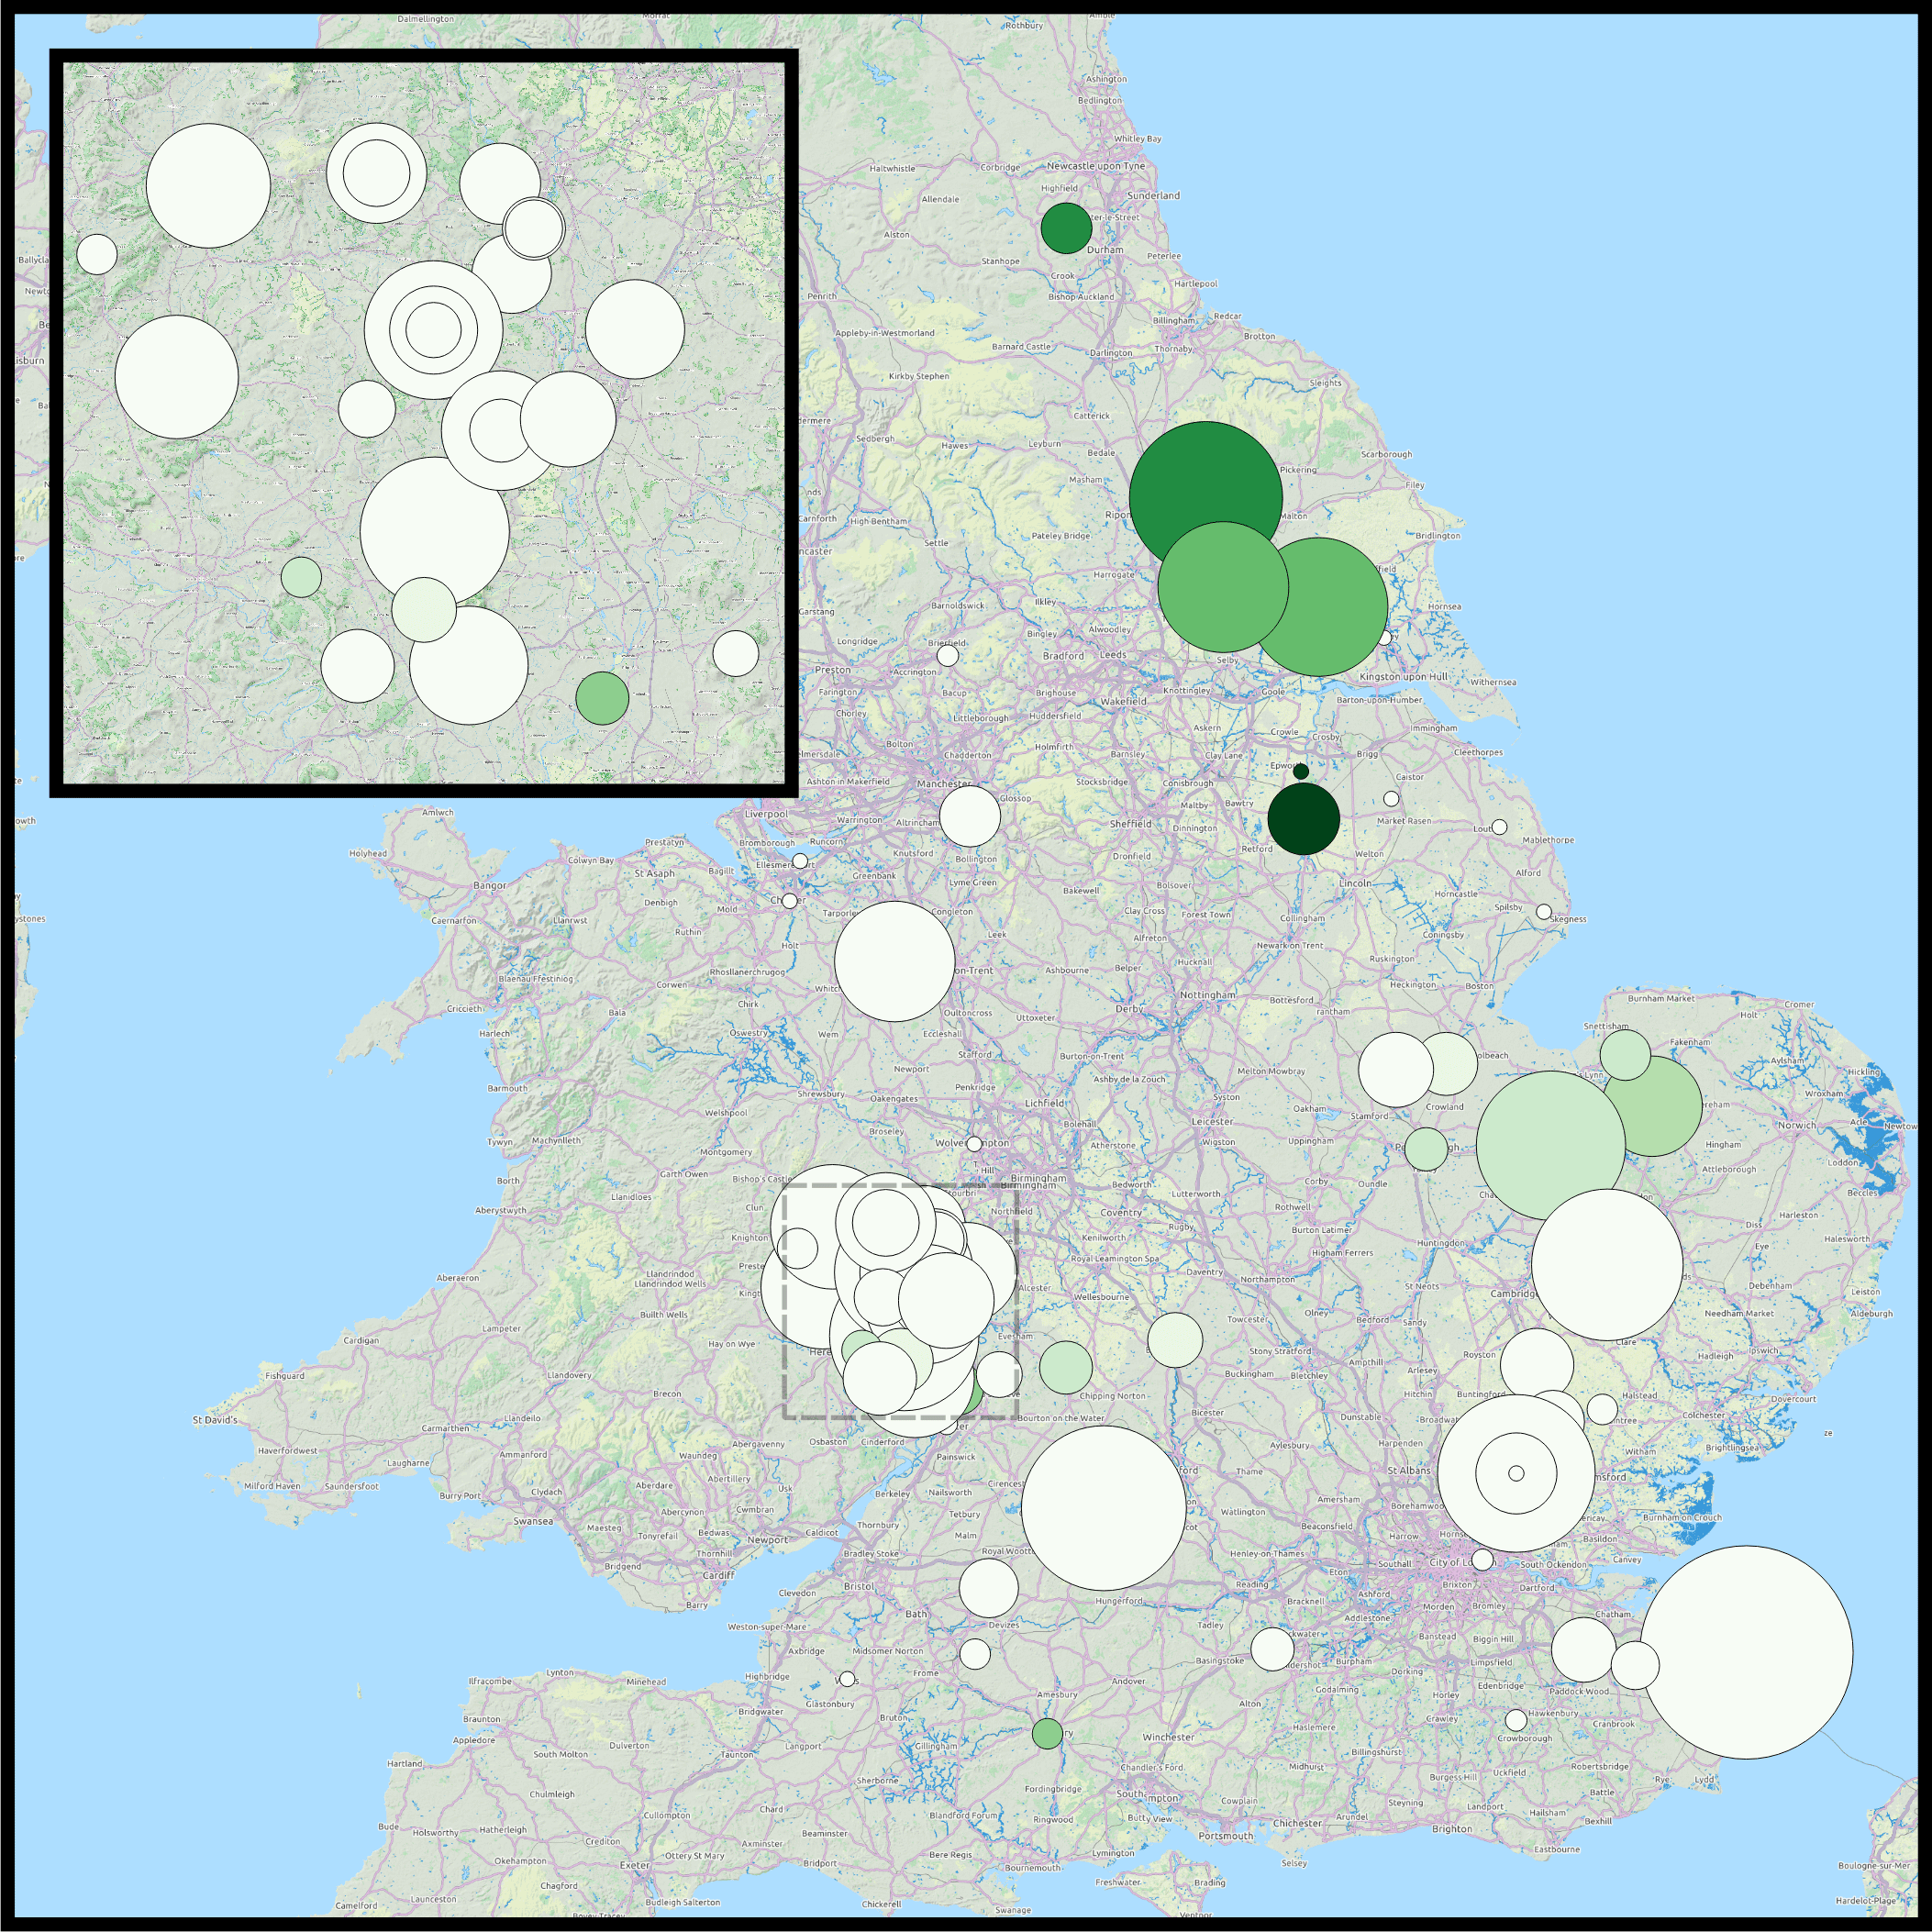
\includegraphics[scale=0.082]{chapters/img/negation-overview.png}
    \caption{Negation in Middle English 1150--1350 \citep[182]{WalkdenMorrison2017}. Darker green points indicate more use of Stage 3.}
    \label{fig:OE-ME-negation}
\end{figure}

\citet{WalkdenMorrison2017} look at the regional distribution\is{regional variation} of the variants using the Linguistic Atlas of Early Middle English \citep{LAEME}. They argue that the disappearance of \emph{ne} may be in part due to \ili{Norse} influence, since Stage 3 seems to emerge first in the north and east (Figure \ref{fig:OE-ME-negation}) -- or at least that contact with \ili{Norse} may have accelerated the change.\footnote{Following ideas first proposed in \citet{Iyeiri1992,Iyeiri2001} and \citet{Ingham2008}.}

What's really interesting about this change, though, is that it is something that has happened independently in dozens of languages, including \ili{Berber}, \ili{Breton}, \ili{Burmese}, \ili{Dutch}, English, \ili{Estonian}, \ili{Fɔn}, \ili{German}, Moroccan Arabic,\il{Arabic, Moroccan} Palestinian Arabic,\il{Arabic, Palestinian} \ili{Norse}, and \ili{Welsh}.\footnote{See \citet{WillisLucasBreitbarth2013} for general discussion.} The full pathway of change from Stage 1 to Stage 3 is known as Jespersen's Cycle,\is{Jespersen's Cycle} after the Danish linguist Otto Jespersen,\ia{Jespersen, Otto} who described the change as follows \citep[4]{Jespersen1917}:

\begin{quote}
    The history of negative expressions in various languages makes us witness the following curious fluctuation: the original negative adverb is first weakened, then found insufficient and therefore strengthened, generally through some additional word, and this in its turn may be felt as the negative proper and may then in course of time be subject to the same development as the original word.
\end{quote}

\noindent Jespersen's Cycle\is{Jespersen's Cycle} is one of the strongest indicators we have that language change in general is \emph{not} completely random but rather follows pathways that are in principle predictable. Obviously, predicting change is still very difficult in practice! But we have no reason to think that it should be impossible, in the long run.

For a full overview of the history of negation in English, see \citet{Ingham2013}. There is also discussion in \citet[305--318]{Fischeretal2000}, including how negation should be captured in a syntactic tree.\is{syntactic trees}


\begin{miscbox}{Negative concord in Old English}
\label{sec:OE-concord}
\glossterm{gl-negative-concord}{Negative concord}, the use of multiple negative-marked words in a single clause to express only one semantic negation -- e.g. \emph{I didn't do nothing to no one} rather than standard \emph{I didn't do anything to anyone} -- is frowned upon by prescriptivists\is{prescriptivism} in Present Day English. It's associated with varieties that have historically had low overt \glossterm{gl-prestige}{prestige}\is{prestige} and been discriminated against, such as African American English\il{English, African American} and Alabama English.\footnote{See \citet{Matyiku2011} at \url{https://ygdp.yale.edu/phenomena/negative-concord} for more on negative concord in present-day varieties of English.}\il{English, Alabama} Those pedants who think that this is an uncouth, illogical innovation may be interested to learn that Old English was a negative concord language, as examples like (\ref{ex:OE-concord}) show.

\begin{exe}
    \ex\label{ex:OE-concord}
    \gll \emph{Ne} mæg \emph{nān} man twām hlāfordum þēowian\\
    \textsc{neg} may no man two masters serve\\
    \trans `No man may serve two masters.'\\
    (\emph{West Saxon Gospels}, Matthew 6:24; \citealp[141]{Ingham2013})
\end{exe}

In fact, the vast majority of the world's languages exhibit negative concord \citep{Haspelmath2013}.\is{negation|)}
\end{miscbox}


\subsection{Relative and correlative clauses}\label{OE-relative}\is{relative clauses|(}

In Present Day English, relative clauses can be introduced in a variety of ways:

\begin{exe}
    \ex The book \emph{\textbf{that}} I read \hfill (\emph{that})
    \ex The book \emph{\textbf{which}} I read \hfill (\emph{which})
    \ex The book \emph{\textbf{Ø}} I read \hfill (zero marking)
\end{exe}

\noindent Similarly, in Old English, relative clauses can be introduced in several different ways. First, they can be introduced by a definite article/demonstrative,\is{articles}\is{demonstratives} which then takes the case\is{case} that the gap in the relative clause would take. If it's a direct object, it appears in the accusative, if it's a subject,\is{subjects} it appears in the nominative, and so on.

\begin{exe}
    \ex
    \gll þā twēġen fēt \emph{\textbf{þā}} þēo sāwul habban sċeal\\
    the two feet \textsc{dem.acc.pl} the soul have shall\\
    \trans `the two feet that the soul shall have' \hfill (\emph{Adrian and Ritheus})
\end{exe}

\noindent Secondly, they can be introduced by the particle \emph{þe}. This is like modern English \emph{that}: it's completely morphologically invariant.

\begin{exe}
    \ex
    \gll tō his āgenum ǣþele \emph{\textbf{þe}} he on ġeboren wæs\\
    to his own country \textsc{particle} he in born was\\
    \trans `to his own country which he was born in' \hfill (\iai{Ælfriċ}, \emph{Life of St. Basil})
\end{exe}

\noindent Thirdly, they can be introduced by both an inflected definite article\is{articles} and the particle \emph{þe} together.

\begin{exe}
    \ex
    \gll Se weig \emph{\textbf{se}} \emph{\textbf{þe}} lǣt tō hēofonrīċe\\
    the way \textsc{dem.nom.sg} \textsc{particle} leads to heaven\\
    \trans `the way which leads to heaven' \hfill (\iai{Ælfriċ}, \emph{Catholic Homilies})
\end{exe}

\noindent Relative clauses crop up quite a lot in Old English texts, so it's useful to see what they look like and how they work. As for their history, the use of the inflected demonstrative\is{demonstratives} died out during the early Middle English period at the same time as the inflected demonstrative itself.\is{demonstratives} The modern type of relative clause introduced by \emph{which}, \emph{who}(\emph{m}) and \emph{whose} was introduced later in the Middle English period.

Another related construction is the correlative construction, which you can see in example (\ref{ex:OE-correlative}).

\begin{exe}
    \ex\label{ex:OE-correlative}
    \gll \emph{\textbf{Ðā}} iċ ðā ðis eall ġemunde, \emph{\textbf{ðā}} wundrade iċ swīðe ðāra gōdena wiotena\\
    when I then this all remembered then marvelled I much the.\textsc{gen.pl} good.\textsc{gen.pl} wise-men.\textsc{gen.pl}\\
    \trans `\emph{When} I remembered all of this, \emph{then} I marvelled at the good wise men exceedingly'\\
    (\emph{Preface} to the translation of Pope Gregory's\ia{Gregory (Pope)} \emph{Pastoral Care})
\end{exe}

\noindent Correlative constructions start with a subordinate clause, followed by a full main clause introduced by a \textsc{resumptive} pronoun\is{pronouns} or adverb. Typically, the resumptive is the same as the element that introduces the subordinate clause. In example (\ref{ex:OE-correlative}), the subordinate clause is introduced by \emph{þā} `when', and the main clause is also introduced by \emph{þā}, in this case meaning `then'.

Correlative constructions are not really found in Present Day English, but they are very common in other Indo-European languages such as Hindi and Urdu\il{Hindi/Urdu} to this day. A similar construction is found with a very heavy nominal phrase at the start, followed by a full main clause introduced by a resumptive pronoun,\is{pronouns} as in example (\ref{ex:OE-resumptive}). Here, \emph{se} (the nominative form of the definite article/demonstrative)\is{articles}\is{demonstratives} introduces the heavy nominal phrase, and also introduces the main clause (in the meaning `he' or `that one').

\begin{exe}
    \ex\label{ex:OE-resumptive}
    \gll \emph{\textbf{Se}} God þe mē forġēaf þis gōde ġeþanc, \emph{\textbf{se}} wyle þē ġehȳran\\
    the God who me gave this good thought he will you hear\\
    \trans `\emph{The} God who gave me this good thought, \emph{he} is willing to hear you'\\
    (\iai{Ælfriċ}, \emph{Life of St. Basil})
\end{exe}

\noindent See if you can spot correlative constructions in Old English texts. Again, there are quite a lot of them!\is{relative clauses|)}


\section{Lexicon}\label{OE-lexicon}

\subsection{Word formation: derivation and compounding}\label{OE-wordformation}\is{word formation|(}\is{affixes|(}

Old English made productive\is{productivity} use of a variety of word-formation strategies in order to form new lexical items. Both \glossterm{gl-derivation}{derivation} (the addition of an affix to a free form) and \glossterm{gl-compounding}{compounding} (putting two free forms together) were widely used during this period.

In the verbal domain, prefixes were common. Thus, verbs like \emph{onsacan} `to refute, to deny' were derived from simple verbs like \emph{sacan} `to attack'. The prefix \emph{be}- made intransitive verbs transitive: so \emph{murnan} `to mourn', as in `they were mourning', gave rise to \emph{bemurnan}, as in `they mourned his death'. However, the function of individual prefixes is often difficult to discern, and sometimes they are used interchangeably in different versions of the same text \citep{Ogura1995}. Verbal prefixes were also an exception to the general rule that all Old English words were stressed on the lexical \glossterm{gl-morpheme}{morpheme}, which was often the first syllable\is{stress shift} (see \sectref{prehistory-stress}) -- this probably reflects the fact that these prefixes are \glossterm{gl-grammaticalization}{grammaticalized}\is{grammaticalization} versions of what once were independent words. The system of verbal prefixes was already becoming less productive\is{productivity} in late Old English, and disappeared almost entirely in Middle English \citep{Hiltunen1983,Lutz1997,Elenbaas2007,Thim2012}.


\begin{miscbox}{The prefix \emph{ġe}-}
\is{aspect}
The prefix \emph{ġe}- is found on both nouns and verbs, though has a different meaning with each. On nouns, \emph{ġe}- often adds a notion of collectivity or grouping, e.g. \emph{ġefēra} `comrade'. This nominal \emph{ġe}- is stressed. On verbs, the function of \emph{ġe}- is hard to pin down, but it seems to be associated with perfectivity or resultativity \citep{McFadden2015}. This verbal \emph{ġe}- is unstressed. It's often found with past participles, but not only with past participles, and can occur with all kinds of verb forms.
\end{miscbox}


\noindent The borderline between derivation and compounding is blurred with Old English nominal word-formations, since it's often difficult to tell whether a given element is a suffix or a free form. Cross-linguistically, it's very common for suffixes to originate as \glossterm{gl-grammaticalization}{grammaticalized}\is{grammaticalization} free forms, but it's hard to know where to draw the line. -\emph{liċ}, for instance, is cognate with the noun \emph{līċ} `body', and is used to form adjectives from nouns, e.g. \emph{heofonliċ} `heavenly' from \emph{heofon} `heaven', and \emph{dēofolliċ} `devilish' from \emph{dēofol} `devil'.\footnote{This is where the adjectival use of \textit{-ly} comes from in Present Day English \textit{friendly} and \textit{manly}.} -\emph{dom} is cognate with the noun \emph{dōm} `judgement', and creates abstract nouns, e.g. \emph{þēowdom} `slavery'\is{slavery} from \emph{þēow} `slave'. These endings, and others such as -\emph{ful}, -\emph{lēas} and -\emph{sċip} (the ancestors of modern -\emph{ful}, \linebreak-\emph{less} and -\emph{ship}) are sometimes referred to by Old English scholars as ``suffixoids'' to indicate that we can't be sure whether they are suffixes or free forms. There are, however, also some unambiguous derivational suffixes in Old English, like -\emph{iġ}, which creates adjectives (giving us the Present Day English -\textit{y} suffix, as in \textit{fishy}, \textit{stormy}, and \textit{windy}), and -\emph{ung} and -\emph{nes}(\emph{s}), which create abstract feminine nouns.\is{affixes|)}

Old English is particularly fond of \glossterm{gl-compounding}{compounding}, and this is nowhere more true than in the poetic\is{poetry} texts (see \citealp{Godden1992}). Some compound elements, such as \emph{heaþo}-, \emph{beadu}- and \emph{hilde}- (all relating to `war'), are only found in the poetry, e.g. \emph{heaþohelm} `war-helm' and \emph{hildebil} `battle-blade, sword'. \citet{DavisSecord2016} is a recent and in-depth study of compounding in Old English literature.


\begin{miscbox}{Kennings}\is{kennings}
\is{poetry}
\textsc{Kennings} are a special type of compound or set phrase, used figuratively, and made up of of two parts: a base word and a determinant. The determinant shares its semantic area with the thing that the kenning refers to overall. Kennings include such compound words as \emph{hronrād} `sea' (literally `whale-road') and \emph{merehengest} `ship' (literally `sea-stallion'). Both Old English and Old Norse poetry make liberal use of kennings.\is{word formation|)}
\end{miscbox}


\subsection{Lexical borrowing}\label{OE-borrowing}\is{borrowings|(}
\largerpage[-1]
The majority of the Old English vocabulary was either inherited from Proto-Germanic or built up using the sort of word-formation strategies discussed in the previous section. That doesn't mean that Old English was free of borrowings, however -- far from it! Brythonic Celtic,\il{Celtic, Brythonic} \ili{Latin}, and \ili{Norse} all contributed to the lexicon of Old English to varying degrees.

The number of accepted lexical borrowings from Brythonic Celtic\il{Celtic, Brythonic} into Old English is small. Old English \emph{brocc} `badger' is one clear case, and there are several elements that are often found in place-names, such as \emph{cumb} `valley', \emph{luh} `lake', \emph{torr} `rock, hill'. We can also identify a few words from Old \ili{Irish}: \emph{drȳ} `magician', also found in the derived form \emph{drȳcræft} `sorcery, witchcraft'. Some scholars (e.g. \citealp{Coates2017}) have taken the relative paucity of accepted borrowings as an indication that the contact situation was not nearly as intense as we suggested in \sectref{OE-Celtic}. This isn't a necessary conclusion, though. Given the low status of Brythonic Celtic\il{Celtic, Brythonic} and Celtic-speakers, it makes sense to imagine that words of Celtic origin would have been consciously suppressed by speakers of Old English: they just weren't prestigious enough. The real impact of Celtic on Old English would then have been on areas of the language that are less subject to conscious scrutiny, such as morphosyntax and perhaps phonology -- which fits well with the evidence (recall \sectref{OE-be} on the twofold paradigm\is{paradigms} of \textit{BE}). We shouldn't expect all language contact situations to have the same outcome.\footnote{For more detail on different outcomes of language contact, see \citet{Winford2005} on `borrowing' vs. `imposition', and \citet{Trudgill2011} on short-term vs. long-term contact situations.} Also, recently it has been suggested that more words were borrowed into Old English from Celtic than previously thought \citep{Breeze2002}, though time will tell whether these etymologies become accepted by the scholarly community.

Direct \ili{Latin} borrowings in Old English are numerous: probably around 600 in total \citep[100]{Durkin2014}. We can often use linguistic evidence, such as the presence or absence of certain sound changes, to determine when exactly a word was borrowed: see \sectref{prehistory-borrowing} in the next chapter for discussion of this and of very early borrowings. Borrowings into Old English itself, after the year 600, mostly had to do with religion and learning, for instance \emph{dēmōn} `demon', \emph{pāpa} `pope', \emph{circul} `circle', and \emph{þēater} `theatre'.\is{Christianity}

There are also very many words which are not direct borrowings but either contain \ili{Latin} elements or are modelled directly on \ili{Latin} morphological structures. In \emph{grammatic-cræft} `grammar', the first element is from \ili{Latin}, but the second element -\emph{cræft} is inherited, and is a productive\is{productivity} way of forming abstract nouns in Old English. The word \emph{ælmihtiġ} `almighty' is almost certainly a loan translation from \ili{Latin} \emph{omnipotens}: in both words the first part (\emph{æl}-, \emph{omni}-) means `all', and the second part (-\emph{mihtiġ}, -\emph{potens}) means `powerful' \citep[164]{Durkin2014}. It's hard to know how many of these borrowings which we find in texts were `real' in the sense of being widely used in speech, rather than opportunistic coinages of the moment. Remember that the texts are heavily biased towards the domains of religion and learning anyway (\sectref{OE-texts}). But it isn't doubted that \ili{Latin} had a major lexical impact on Old English. See \citet[part III]{Durkin2014} for extensive discussion.

\ili{Norse} borrowings into English are also very numerous. They start to appear only in late Old English (see \sectref{OE-Scandinavian}), and at this point are mostly restricted to specific domains: seafaring (e.g. \emph{barþ} and \emph{cnear}, types of ship), law\is{legal language} (e.g. \emph{lagu} `law' itself!), warfare (e.g. \emph{grið} `peace'). \citet{PonsSanz2013} lists 185 accepted \ili{Norse} borrowings in Old English, and many more that are disputed. During the Middle English period, more \ili{Norse} borrowings flow into the language, including many that are still used today: \emph{die}, \emph{egg}, \emph{meek}, \emph{though}. \citet{Townend2002} points out that the borrowings from \ili{Norse} into Old English tend to show signs of adaptation to Old English phonology, whereas the later borrowings first attested in Middle English do not. This could indicate a general change in the nature of the contact situation, away from \glossterm{gl-prestige}{prestige}-driven\is{prestige} borrowing and towards substitution of everyday words -- perhaps by native speakers of \ili{Norse}, as the language slowly died out in England during the Middle English period.

\newpage
At present, \citet{PonsSanz2013} is the definitive overview of \ili{Norse} borrowings into Old English. \citet[part IV]{Durkin2014} discusses Scandinavian lexical influence in general, and the Gersum Project website allows you to look up potential borrowings and how likely it is that they truly have \ili{Norse}\is{borrowings|)} origins.\footnote{Available at \url{https://www.gersum.org}.}

\section{Final note}

Old English is a challenge for the reader, especially if -- as will be the case for most students using this book -- this is the first time you're encountering it. But don't worry: no one is expecting you to become fluent! Instead, just give your curiosity free rein and explore this weird and wonderful period of the English language with an open mind.

We've focused in this chapter on the multilingual\is{multilingualism} nature of early Britain. English was just one language among many during this period, and it would have been impossible to predict with any confidence in 600, 1000 or 1150 that it would eventually become the most widely spoken language in Britain (still less the world). Old English coexisted with Brythonic Celtic, Norse, Latin, and later French. It wasn't just Britain as a whole that was multilingual; individuals of all social classes very often spoke more than one language, and the development of English from 600 onwards reflects this coexistence of languages.\is{multilingualism}


\addsec{Suggested exercises}

\begin{exercises}{Letters vs. sounds}\label{exercise-OE-spelling}
What are the Present Day English equivalents of the following Old English words? Don't use a dictionary\is{dictionaries} -- simply guess. The Old English words below all happen to be very similar to their Present Day English equivalents, so don't expect any treacheries here: if \textit{ofer} looks like the Present Day English \textit{over} to you, assume that this is indeed what it is.

Comment on the spelling\is{orthography} and the pronunciation differences. 
\clearpage

\begin{multicols}{2}
\begin{enumerate}
  \item æsc
  \item bedd
  \item cynn
  \item dæg
  \item fisc
  \item hyll
  \item mann
  \item miht
  \item ofer
  \item scip
  \item ðorn
  \item þorn
  \item þynn
\end{enumerate}
\end{multicols}
				
\noindent This exercise is adopted and adapted from \citet{HoggAlcorn2012}.

\end{exercises}

\begin{exercises}{Pronouncing Old English}\label{exercise-OE-pronounce}
How about trying to transcribe the first line of \textit{Beowulf} in the International Phonetic Alphabet?\\

\textit{Hwæt wē gārdena in ġēardagum}\\


\subsection{Using the Bosworth-Toller Dictionary}
The Bosworth-Toller Dictionary\is{dictionaries} by Joseph Bosworth\ia{Bosworth, Joseph} and T. Northcote Toller is available online for you to use.\ia{Toller, Thomas Northcote}\footnote{Available at \url{https://bosworthtoller.com/}. Digitalized by Sean Crist and Ond\v{r}ej Tich\'{y}, maintained by Ond\v{r}ej Tich\'{y}.} It's a fantastic source to use when you need to look up an Old English word. However, it may take a while to orientate oneself when first using it. This should become a bit easier by following these tasks:

\begin{enumerate}
  \item Look these words up: \textit{cearu}, \textit{lic} (the very first entry), \textit{loða}, \textit{scitan} (the second entry), \textit{werewulf}, and \textit{wifmann}.
  \item What information does the dictionary provide you with when it comes to these words? Is it useful?
  \item Now try something like \textit{durste}. The search will give you useful information, but you'll have to do a bit more hunting in this case to get to know what \textit{durste} means exactly. Can you figure out how?
\end{enumerate}

\noindent\emph{Hint:} the rather mysterious abbreviations such as \textit{an} and \textit{es} provide you with the ending representing the genitive singular. The \textit{f.}, \textit{m.}, and \textit{n.} abbreviations give you information on the morphological gender\is{gender (grammatical)} of the noun in question.\\

\noindent\emph{Tip for teachers:} Go through the less obvious parts of the dictionary\is{dictionaries} with the students, such as the links to the paragraphs of the Wrights'\ia{Wright, Joseph}\ia{Wright, Elizabeth Mary} \textit{Old English Grammar} with the \textit{lic} entry.

\end{exercises}

\begin{exercises}{Fricative allophony}\label{exercise-OE-fricatives}\is{voicing allophony}
Old English did not have voiced and voiceless fricatives as contrasting \glossterm{gl-phoneme}{phonemes}. [f] and [v], [s] and [z], and [θ] and [ð] did exist, but as conditioned \glossterm{gl-allophone}{allophones}. Sort the following words into two categories, deciding whether the letter in bold represents a voiceless or a voiced fricative in the pronunciation. 

% \begin{multicols}{6}
% \begin{tabular}{cc}
\TabPositions{.2\textwidth,.6\textwidth,.8\textwidth}
% \lsptoprule
%  OE \tab  PDE translation\tab
%  \midrule

\noindent
 \textbf{s}æ \tab  `sea' \tab
 bro\textbf{ð}or \tab  `brother' \tab
 wi\textbf{f} \tab  `wife, woman' \tab
 hræ\textbf{f}n \tab  `raven' \tab
 \textbf{f}lota \tab  `ship' \tab
 cea\textbf{s}ter \tab  `city' \tab
 weor\textbf{þ}e \tab  `worthy' \tab
 o\textbf{f}er \tab  `over' \tab
 ri\textbf{s}an \tab  `to rise' \tab
 æ\textbf{þ}ele \tab  `noble' \tab
 ly\textbf{f}t \tab  `air' \tab
 yrh\textbf{ð}o \tab  `slackness' \tab
%  \lspbottomrule
% \end{tabular}
%
% \begin{tabular}{cc}
% \lsptoprule
%  OE \tab  PDE translation\tab
%  \midrule
 of\textbf{f}rian \tab  `to offer' \tab
 bo\textbf{s}om \tab  `bosom' \tab
 oð\textbf{ð}e \tab  `or' \tab
 wæ\textbf{s} \tab  `was' \tab
 \textbf{þ}egn \tab  `thane' \tab
 e\textbf{f}ne \tab  `even' \tab
 no\textbf{s}u \tab  `nose' \tab
 bli\textbf{þ}e \tab  `joyous, blithe' \tab
 heo\textbf{f}on \tab  `heaven' \tab
 hæ\textbf{s}len \tab  `of hazel' (adj)\tab
 be-\textbf{s}ecgan \tab  `to announce' \tab
%  \lspbottomrule
% \end{tabular}
% \end{multicols}

\noindent\emph{Note:} voiced sounds include vowels,\is{vowels} liquids, nasals, and all voiced stops.\\

\noindent\emph{Note:} all the spellings\is{orthography} with two graphemes e.g. <ff> count as two separate ``sounds''/sound events/segments.\\

\noindent\emph{Note:} the allophonic voicing rule didn't operate across morphemes, i.e. it was blind to the vowels\is{vowels} and consonants\is{consonants} that were not part of the morpheme in which we find the relevant fricative.\is{voicing allophony}\\

\noindent\emph{Acknowledgement:} this exercise is adapted from Johanna Wood's\ia{Wood, Johanna L.} 2016 teaching materials.

\end{exercises}

\largerpage[3]
\begin{exercises}{Identifying nominal features}\label{exercise-OE-nominalmorph}

For each of the following phrases, identify the case,\is{case} number, gender,\is{gender (grammatical)} and class of the noun. If there is more than one possibility for case or gender, list all the possibilities. Try not to use a dictionary.\is{dictionaries}

\begin{enumerate}
    \item \emph{þone bāt} (noun: `boat')
    \item \emph{þā dōru} (noun: `door')
    \item \emph{sēo faru} (noun: `journey')
    \item \emph{þæs flēogan} (noun: `fly')
    \item \emph{þāra ēagena} (noun: `eye')
    \item \emph{þone docgan} (noun: `dog')
    \item \emph{þā huniġcambe} (noun: `honeycomb')
    \item \emph{þǣm dorum} (noun: `bee')
\end{enumerate}

\end{exercises}

\begin{exercises}{Murder mystery}\label{exercise-OE-murder}
In this exercise, you'll be learning about Old English morphology using the following nouns as our practice material: 

\begin{center}
\begin{tabular}{c@{}ccc}
 \lsptoprule
 \textbf{PDE} & \textbf{OE nominative} & \textbf{OE genitive} & \textbf{OE accusative}\\
 \midrule
 `chief' & fruma & fruman & fruman \\
 `friend' & freond & freondes & freond \\
 `lady (of the house)' & hlæfdige & hlæfdigan & hlæfdigan\\
 \lspbottomrule
\end{tabular}
\end{center}

\noindent Now here's the murder mystery (more or less in Present Day English). The main protagonists are presented to you in Old English and you can't rely on the word order\is{word order} to know who did what to whom. You have to rely on the morphology. Below are three questions you need to answer.

\begin{quote}
    Once a \emph{fruma} was a guest in a \emph{freondes} hall. His \emph{freond} went out to hunt. The \emph{fruma} the \emph{hlæfdigan} regarded (looked at). The \emph{fruman} the \emph{hlæfdige} regarded. Followed the \emph{hlæfdigan} the \emph{fruma}. The \emph{hlæfdige} the \emph{fruman} feared. Desired the \emph{hlæfdigan} the \emph{fruma}.  The \emph{fruman} fled the \emph{hlæfdige}. Embraced the \emph{hlæfdigan} the \emph{fruma}. The \emph{fruman} the \emph{hlæfdige} insulted. Twisted the \emph{hlæfdigan} arm the \emph{fruma}.  Kicked the \emph{fruman} the \emph{hlæfdige} where it hurts real bad. Hit the \emph{fruma} the \emph{hlæfdigan}. The \emph{fruman} the \emph{hlæfdige} slew.
\end{quote}

\noindent Answer these questions:
\begin{enumerate}
    \item Who is lying dead on the floor?
    \item Who did it?
    \item Why?
\end{enumerate}

\noindent\emph{Acknowledgement:} we inherited this exercise from Johanna Wood\ia{Wood, Johanna L.} and Ocke-Schwen Bohn;\ia{Bohn, Ocke-Schwen} however, we have not been able to trace the author of this wonderful activity.

\end{exercises}

\begin{exercises}{Irregular plurals}\label{exercise-OE-plurals}\is{irregularities}
A. \newline
\noindent There are various strategies to form the plural\is{plurals} in Present Day English. The regular strategy is to add the -\emph{(e)s} morpheme to the singular form, as in \emph{bumblebee} > \emph{bumblebees}.\is{bumblebees} Was this the case in Old English?\\

\noindent B. \newline
\noindent The singular/plural pairs below use a different strategy and have to be learnt as exceptions to the regular plural\is{plurals} rule in Present Day English. Using the Magic Sheet, say which Old English morphological classes the following Present Day English irregular\is{irregularities} plurals\is{plurals} derive from:

\begin{enumerate}
  \item \textit{sheep} $\sim$ \textit{sheep}
  \item \textit{man} $\sim$ \textit{men}
  \item \textit{deer} $\sim$ \textit{deer}
  \item \textit{fish} $\sim$ \textit{fish}
  \item \textit{knife} $\sim$ \textit{knives}
  \item \textit{ox} $\sim$ \textit{oxen}
  \item \textit{wolf} $\sim$ \textit{wolves}
\end{enumerate}

\noindent C. \newline
\noindent Identify the origin of the irregularity\is{irregularities} for each of the following pairs.

\begin{enumerate}
  \item \textit{tooth} $\sim$ \textit{teeth}
  \item \textit{louse} $\sim$ \textit{lice}
  \item \textit{child} $\sim$ \textit{children}\footnote{\textit{Children} are difficult. You probably won't be able to explain the entire plural\is{plurals} form, but give it a go.}
\end{enumerate}

\noindent \emph{Note:} the whole point is for you to be able to identify the historical source of these Present Day English irregularities.\is{irregularities} We don't expect you to remember what the different classes should/can be labelled exactly, but we do expect you to know where to look in the Magic Sheet.

\noindent \emph{Acknowledgement}: This exercise was partly inspired by Johanna Wood's 2016 teaching materials.\ia{Wood, Johanna L.}

\end{exercises}

\begin{exercises}{Contrasting Present Day English with Old English}\label{ex-OE-PDE}

Below are extracts from \textit{The Wanderer}. You are provided with the corresponding Present Day English translations. Your task is to explain how the expressions in bold differ from their Present Day English equivalents in terms of their syntax and verbal morphology.

Using the digital version of the Bosworth-Toller Dictionary\is{dictionaries} will be helpful if you work with Old English.\footnote{\url{https://bosworthtoller.com/}.}\\

\noindent \textit{The Wanderer}:\footnote{Adapted from Miller (\url{http://www.anglo-saxons.net/hwaet/?do=get&type=text&id=Wdr}).}

\begin{center}
\begin{tabular}{ cc }
\lsptoprule
 Old English & Present Day English \\
 \midrule
 Oft \emph{\textbf{him (1)}} \emph{\textbf{anhaga (2)}} & Often \emph{\textbf{the solitary one (2)}}\\ 
 \emph{\textbf{are gebideð (3)}}, &\emph{\textbf{finds grace (3)}} for \emph{\textbf{himself (1)}},\\ 
 \emph{\textbf{metudes miltse (4)}}, &\emph{\textbf{the mercy of the Lord (4)}},\\
 þeah þe he modcearig &Although he, sorry-hearted,\\
 geond lagulade &through sea ways\\
 longe \emph{\textbf{sceolde hreran (5)}} &long \emph{\textbf{should row (5)}}\\
 \emph{\textbf{mid hondum (6)}} &\emph{\textbf{with hands (6)}}\\
 hrimcealde \emph{\textbf{sæ (7)}}, &the ice-cold \emph{\textbf{sea (7)}},\\
 wadan wræclastas. &tread the paths of exile.\\
 Wyrd bið ful aræd! &Fate is fully determined!\\
 \emph{\textbf{Swa cwæð eardstapa (8)}}, &\emph{\textbf{The wanderer spoke so (8)}},\\
 \emph{\textbf{Earfeþa gemyndig (9)}}, &\emph{\textbf{mindful of hardships (9)}},\\
 wraþra wælsleahta, &of fierce slaughters,\\
 winemæga hryre &	and the downfall of kinsmen.\\
 \lspbottomrule
\end{tabular}
\end{center}

\end{exercises}

\begin{exercises}{Verb phrases}\label{exercise-OE-VPs}

Translate the following clauses into Present Day English. Use a dictionary\is{dictionaries} where you need to. For each of them, say whether the verb phrase in Old English is head-initial or head-final. Remember: the non-finite verb is crucial!

\begin{enumerate}
    \item Ac hē sċeal þā sacfullan ġesibbian
    \item þæt hē ne mæġe nān gōd dōn
    \item se wolde ofslēan þone cyning Dauid
    \item ġif hēo þæt bysmor forbēran wolde
    \item ðæt hē wolde ġenealæcan his hulce
\end{enumerate}

\end{exercises}

\begin{exercises}{Emphasizing negation}\is{negation|(}
When you read about Jespersen's\ia{Jespersen, Otto} Cycle\is{Jespersen's Cycle} in this chapter, you learnt about \textit{not} having evolved out of what used to be added on top of the negative \textit{ne} for emphatic reasons, as in the Present Day English \textit{The bumblebee did\textbf{n't} give a \textbf{hoot} about all the blossoms}. There are plenty of words of the \textit{hoot} type that we use today to emphasize negation. One more example would be \textit{The bumblebee\is{bumblebees} did\textbf{n't} give a \textbf{fig} about all the blossoms}. 

\newpage
Using your own knowledge of English, asking other speakers, and/or searching online, how many other such \textit{hoot} type words can you come up with? Aim for as many as possible. Do these have the same meaning, would you say?\is{negation|)}

\end{exercises}

\begin{exercises}{Change across Old English}
Look at the two excerpts from the \textit{Peterborough Chronicle} in \sectref{OE-chronicle} below. The first presents an older stage of Old English, the latter presents a newer stage of Old English (in fact, very early Middle English according to where we've drawn the line). Which linguistic differences suggest that the former is older and the latter is younger?

\end{exercises}

\begin{exercises}{Translating \textit{Beowulf}}
\chili{}
A.\is{poetry|(} Comment on the following remark Heaney\ia{Heaney, Seamus} has made on his translation of \textit{Beowulf} regarding his use of Irishisms \citep[xxxiv]{Heaney2000}:

\begin{quote}
    [...] I have in several instances used the word `bawn' to refer to Hrothgar's hall. In Elizabethan English, bawn (from the \il{Irish} \textit{bó-dhún}, a fort for cattle) referred specifically to the fortified dwellings which the English planters built in Ireland to keep the dispossessed natives at bay [...]. Putting a bawn into \textit{Beowulf} seems one way for an Irish poet to come to terms with that complex history of conquest and colony, absorption and resistance, integrity and antagonism, a history which has to be clearly acknowledged [...].
\end{quote}

\noindent What are the pros and cons of this approach to translating \textit{Beowulf}?\\

\noindent B. Old English poetry employed certain linguistic structures in ways in which these are no longer used in present-day English. One of these differences is the very frequent use of \glossterm{gl-compounding}{compounding}\is{word formation} in Old English poetry. On this, \citet[xxxiii]{Heaney2000} says the following:

\begin{quote}
Old English abounds in vigorous and evocative and specifically poetic words for these things [i.e. a sword or a spear or a battle or any bloody encounter with foes], but I have tended to follow modern usage and in the main have called a sword a sword.
\end{quote}

\noindent Would you support Heaney's\ia{Heaney, Seamus} decision to ``call a sword a sword'', so to speak, in a Present Day English rendition of the poem? Why (not)?\\

\noindent C. Here we present you with two passages from the poem: one in Old English (OE), one being a philological translation serving as a maximally detailed type of glossary (PT), and the translation by Seamus Heaney (SH).\ia{Heaney, Seamus}\\


\emph{Encounter with Grendel's mother:}
\begin{quote}
OE: Ongeat þa se goda grund-wyrgenne\\
OE: mere-wif mihtig; mægen-ræs forgeaf\\
OE: hilde-bille, hond sweng ne ofteah,\\
OE: þæt hire on hafelan hring-mæl agol\\
OE: grædig guð-leoð.\\
\citep[104]{Heaney2000}
\end{quote}

\begin{quote}
PT: Perceived [he] then the good ground-throttler\\
PT: mare-wife [= woman] mighty; might-rush [he] gave\\
PT: slope-edged, hand blow not spared [i.e. he didn't spare],\\
PT: it [i.e. the sword] her on head ring-ornamented sang\\
PT: greedy battle-poem/song.
\end{quote}

\begin{quote}
SH: The hero observed that swamp thing from hell,\\
SH: the tarn-hag in all her terrible strength,\\
SH: then heaved his war-sword and swung his arm:\\
SH: the decorated blade came down ringing\\
SH: and singing on her head.\\
\citep[105]{Heaney2000}
\end{quote}

\emph{Having killed the dragon:}
\begin{quote}
OE: Nalles æfter lyfte lacende hwearf\\
OE: middel-nihtum, maðm-æhta wlonc\\
OE: ansyn ywde; ac he eorðan gefeoll\\
OE: for ðæs hild-fruman hond-geweorce.\\
\citep[190]{Heaney2000}
\end{quote}

\begin{quote}
PT: Not-at-all after in the air playing [he] turned\\
PT: [at] midnight, of costly-possesions proud\\
PT: face showed; and he to earth fell\\
PT: for [= by] that war-ruler hand-work
\end{quote}

\begin{quote}
SH: Never again would he glitter and glide\\
SH: and show himself off in midnight air,\\
SH: exulting in his riches: he fell to earth\\
SH: through the battle-strength in Beowulf's arm.\\
\citep[191]{Heaney2000}
\end{quote}

\noindent And here are your tasks:
\begin{itemize}
\item How much does Seamus Heaney\ia{Heaney, Seamus} diverge from the original?
\item When he diverges, what consequences does this have for the reader of the literary work?
\item Why not try a translation of your own?
\end{itemize}

\noindent D. Look at the two passages above. Compare the Old English version with the Present Day English version from a purely linguistic point of view. How has the language changed since the times of \textit{Beowulf}? Why is Old English challenging for a Present Day English speaker?\\

\noindent E. If you have access to the following review of Heaney's\ia{Heaney, Seamus} \textit{Beowulf},

\begin{quote}
    Čermák, Jan. \citeyear{Cermak2012}. Heaney's Beowulf: gleaning the unsaid off the palpable. In Jana K. Schulman\ia{Schulman, Jana K.} \& Paul E. Szarmach\ia{Szarmach, Paul E.} (eds.), \emph{Beowulf at Kalamazoo: essays on translation and performance}, 301--304. Michigan: Medieval Institute Publications.
\end{quote}

\noindent Focus on the following:
\begin{itemize}
\item What differences between the two versions of the poem does Čermák list? 
\item Are these important differences? Why (not)?
\end{itemize}

\noindent \emph{Tips for teachers:} give the students a word limit and a deadline to submit a summary if a written type of exercise is seen as helpful.

\end{exercises}

\begin{exercises}{Ezra Pound's translation of \textit{Seafarer}}
\chili{}
Below are the first seven lines of the \textit{Seafarer}. We provide you with the Old English transliteration (``OE''),\footnote{Page 306 here: \url{https://archive.org/details/codexexoniensisc00sociuoft/page/306}.} a philological translation serving as a maximally detailed type of glossary (PT), and a translation by Ezra Pound\ia{Pound, Ezra} (EP).\footnote{\url{https://www.poetryfoundation.org/poems/44917/the-seafarer}.}

\begin{quote}
OE: maeg ic be me sylfum\\
OE: soðgied wrecan\\
OE: siþas secgan\\
OE: hu ic geswincdagum\\
OE: earfoðhwile\\
OE: oft þrowade\\
OE: bitre breostceare
\end{quote}

\begin{quote}
PT: may I by me [= my] self\\
PT: a true tale work [= make]\\
PT: travels say\\
PT: how I at days of labour\\
PT: a time of hardship\\
PT: oft suffered\\
PT: bitter breastcare [= sorrow, anxiety]
\end{quote}

\begin{quote}
EP: May I for my own self\\
EP: song's truth reckon\\
EP: Journey's jargon,\\
EP: how I in harsh days\\
EP: hardship\\
EP: endured oft\\
EP: Bitter breast-cares have I abided
\end{quote}

\noindent And here are your tasks:
\begin{itemize}
\item How much does Ezra Pound\ia{Pound, Ezra} diverge from the original?
\item When he diverges, what consequences does this have for the reader of the literary work?
\item Why not try a translation of your own?\is{poetry|)}
\end{itemize}

\end{exercises}

\begin{exercises}{Food for thought}
Engage with the following statements. Argue for and/or against:

\begin{itemize}
  \item Contrasting Old English and Present Day English spelling reveals some important sound changes that have happened in the history of English.\is{orthography}
  \item Old English morphology was so different from Present Day English morphology that one could argue Old English and Present Day English are two different languages.
  \item Old English had a free word order.\is{word order}
  \item We cannot approach Old English from a sociolinguistic\is{sociolinguistics} point of view.

  \newpage
  \item The Middle English words <veal>, <vertú>, and <Zephirus> are very likely to be inherited from Old English.
\end{itemize}

\noindent \emph{Tip for teachers:} Assign one of these questions as a written exercise, giving the students a word count limit and a deadline.

\end{exercises}

\begin{exercises}{Improve these statements}\label{ex-OE-statements}
Could you improve the following claims in any way?
\begin{itemize}
  \item ``Nouns in Old English were gendered.''\is{gender (grammatical)}
  \item ``The Present Day English \textit{hardly} gained the derivational suffix\is{affixes} -\textit{ly}, which now shows its grammatical case\is{case} as an adverb.''
  \item ``English was influenced by Germanic.''
  \item ``The tense of \textit{cuman} is the plural\is{plurals} form of \textit{cuma}.''
  \item ``Throughout its history, English has lost a lot of casing.''
  \item ``The Old English prefix\is{affixes} \textit{ge-} was inherited from earlier forms of \ili{German} and \ili{Dutch}.''
  \item ``V2\is{verb-second} refers to the free word order we find in Old English, where the verb occurs at the end of a sentence.''\is{word order}
  \item ``The Old English case\is{case} can also determine the mood of the verb.''
  \item ``The Old English verb \textit{biddeþ} has the thorn\is{thorn} as a suffix.''\is{affixes}
\end{itemize}
\end{exercises}


\addsec{Text samples}
Below we have prepared a choice selection of Old English texts for you. \iai{Wulfstan}'s \textit{Sermo Lupi ad Anglos} presents a late Old English text, as does the poem\is{poetry} \emph{Judith}. \emph{Wulf and Eadwacer} is a female-voiced poem, and the \emph{Voyage of Ohthere}\ia{Ohthere} sheds light on relations between Scandinavians and Old English speakers. The two excerpts from the \emph{Chronicle} provide a window onto narrative history-telling of the period, centuries apart. As usual, the texts are in reverse chronological order, but you might like to start with the excerpt of the Life of St Basil in \sectref{OE-lives}, for which we've provided full glossing and translation.

In the next chapter you'll find a couple more early Old English texts, including \textit{The Law of Æþelberht}\ia{Æþelberht (King of Kent)}.


\begin{texts}{Wulfstan's \textit{Sermo Lupi ad Anglos}}
\iai{Wulfstan} was an important ecclesiastical figure of the British world of the end of the 10th and the beginning of the 11th centuries. His \textit{Sermo Lupi ad Anglos} translates into `Wolf's Sermon to the English' and is an early 11th-century homily, in which \iai{Wulfstan} blames the Scandinavian incursions on the moral decline of the English. Below we give you an excerpt of this best-known of \iai{Wulfstan}'s works.\footnote{From the manuscript\is{manuscripts} at \url{http://www.bl.uk/manuscripts/Viewer.aspx?ref=cotton_ms_nero_a_i_f070r}, MS Cotton, Nero, A 1, ff. 111v--112r; accessed May 2020; original punctuation preserved; overdotting and length marking added; abbreviations silently expanded.}

\begin{quote}
    \internallinenumbers*{}
    Ne ǣniġ ƿið ōþerne \.{ʒ}etrȳƿlīċe · sƿā rihte sƿā hē scolde · ac mǣst ǣlċ swicode · ⁊ōþrum derede · ƿordes ⁊dǣde· ⁊hūru unrihtlīċe mǣst ǣlċ ōþerne æftan hēaƿeþ. mid sceandlican onscytan · dōmāre \.{ʒ}if hē mæ\.{ʒ}e · forþām hēr syn onlande un\.{ʒ}etrȳƿþa miċle · forʒode ⁊for ƿorolde·⁊ eac hērsyn on earde on mistliċe ƿīsan · hlāford sƿican mane\.{ʒ}e; ⁊ealra mǣst hlāfordsƿice sebið onƿorolde· þæt man his hlāfordes sāule besƿīce; ⁊ful miċel hlāford sƿice ēac bið onƿorolde · þæt man his hlāford· of līfe for rǣde; Oððonoflande lifiendne drīfe; ⁊ǣ\.{ʒ}þer is \.{ʒ}eƿorden · on þysan earde;Ēad ƿeard man for rǣdde · ⁊syððan ācƿealde· ⁊æfter þām forbærnde;
    %\end{linenumbers}
\end{quote}


\end{texts}

\begin{texts}{\textit{Judith}}\is{poetry|(}
\textit{Judith} is a late 10th -- early 11th-century Old English poem, which depicts a female character as one of the main protagonists and certainly as a heroine figure. Below we provide you with the excerpt describing how Judith beheaded the Assyrian general Holofernes in his drunken sleep.\footnote{From the Cotton MS Vitellius A XV manuscript\is{manuscripts} at \url{http://www.bl.uk/manuscripts/Viewer.aspx?ref=cotton_ms_vitellius_a_xv_f094r}, ff. 204v–205r; accessed May 2020; original punctuation preserved; overdotting and length marking added; silent abbreviations expanded. We follow the line numbering found here (and elsewhere): \url{http://www.oldenglishaerobics.net/judith.php} for ease of comparison.}

\begin{quote}
    %\begin{linenumbers}[94]
    hī ðā se hēhsta dēma\\
    ǣdre mid elne onbryrde     sƿā hē dēð ānra \.{ʒ}ehƿylċne\\
    hērbūendra     þe hyne him tō helpe sēċeð\\
    mid rǣde ond mid rihte \.{ʒ}elēafan     Þā ƿearð hyre rūme on mōde\\
    hāli\.{ʒ}re hyht \.{ʒ}enīƿod     \.{ʒ}enam ðā þone hǣðenan mannan\\
    fæste be feaxe sīnum     tēah hyne folmum ƿið hyre ƿeard\\
    bysmerlīċe     ⁊ þone bealofullan\\
    listum ālēde     lāðne mannan\\
    sƿā hēo ðæs unlǣdan     ēaðost mihte\\
    ƿel ʒewealdan     slōh ðā ƿundenlocc\\
    þone fēondsceaðan     fāʒum mēċe\\
    heteþoncolne     þæt hēo healfne forċearf\\
    þone sƿēoran him     þæt hē on sƿīman læ\.{ʒ}\\
    druncen · ⁊ dolhƿund     næs ðā dēad þā \.{ʒ}ȳt\\
    ealles orsāƿle     slōh ðā eornoste\\
    ides ellenrōf     ōðre sīðe\\
    þone hǣðenan hund     þæt him þæt hēafod ƿand\\
    forð on ðā flōre     læ\.{ʒ} se fūla lēap\\
    ʒēsne beæftan     ʒǣst ellor hƿearf\\
    under neoƿelne næs     ⁊ ðǣr \.{ʒ}enyðerad ƿæs\\
    sūsle \.{ʒ}esǣled     syððan ǣfre\\
    ƿyrmum beƿunden     ƿītum \.{ʒ}ebunden\\
    hearde \.{ʒ}ehæfted     in helle bryne\\
    æfter hinsīðe     ne ðearf hē hopian nō\\
    þȳstrum forðylmed     þæt hē ðonan mōte\\
    of ðām ƿyrmsele     ac ðǣr ƿunian sceal\\
    āƿa tō aldre     būtan ende forð\\
    in ðām\footnote{Expanded here from the original <ðū>.} heolstran hām     hyhtƿynna lēas·\is{poetry|)}
    %\end{linenumbers}
\end{quote}


\end{texts}

\begin{texts}{\textit{Lives of Saints}}\label{OE-lives}\is{Christianity}
\iai{Ælfriċ}'s \textit{Lives of Saints} were written in the 990s. They're usually classed as prose texts, but are regularly rhythmical and alliterative,\is{alliteration} showing that the boundary between poetry\is{poetry} and prose is not a hard-and-fast one. For texts at the height of piety, some scurrilous and shocking activities are described! We've added glossing and translation to this extract from the Life of St Basil to make your entry into Old English text-reading a bit easier at least here.\footnote{From Skeat's\ia{Skeat, Walter W.} edition at \url{https://en.wikisource.org/wiki/Ælfric\%27s_Lives_of_Saints}; accessed May 2020; glossing, overdotting and length marking added.}

\begin{quote}
    \gll Sum ārƿurþe þeġn hæfde āne dohter · þā hē ƿolde ġebringan · binnan sumum mynstre · ⁊ criste be-tæcan · to his clænan þēoƿdome · þā ƿearð an his cnapena · to cūð þām mǣdene · ⁊ þurh dēofles tihtinge · hī dīgolliċe lufode · ac hē ne dorste āmeldian his unġemetegodan lufe · Ēode þā to anum drymen þe deofles cræft cūðe · ⁠⁊ behēt him sceattes · ġif hē mid his scȳn-cræfte him þæt mǣden mihte ġe-macian to ƿīfe · Þa ge-brohte se dry-man · þone cnapan · tō his dēofle · ⁠⁊ se dēofol befrān · þone dƿeligendan cnapan · ġif hē ƿolde on hine gelȳfan · ⁊ his hælende ƿiðsacen · ƿið þā þe hē ġefremode his fūlan gālnysse ·\\
    an honourable thane had a-\textsc{acc} daughter ~ when he wanted bring-\textsc{inf} ~ within a monastery ~ and Christ-\textsc{dat} show-\textsc{inf} ~ to his pure servitude ~ then became one his boy-\textsc{gen.pl} ~ tō known the.\textsc{dat} maiden-\textsc{dat} ~ and through devil-\textsc{gen} persuasion ~ her.\textsc{acc} secretly loved ~ but he \textsc{neg} dared make.known-\textsc{inf} his unmoderated love ~ went then to a-\textsc{dat} sorcerer-man.\textsc{dat} \textsc{particle} dēvil-\textsc{gen} power knew ~ and promised him treasure-\textsc{gen} ~ if he with his illusion-power-\textsc{dat} him the maiden might make-\textsc{inf} to wife ~ Then brought the.\textsc{nom} sorcerer-man.\textsc{nom} ~ the.\textsc{acc} boy-\textsc{acc} ~ to his devil-\textsc{dat} ~ and the.\textsc{nom} devil.\textsc{nom} asked ~ the.\textsc{acc} straying boy-\textsc{acc} ~ if he wanted in him believe-\textsc{inf} ~ and his saviour deny-\textsc{inf} ~ against \textsc{dem.acc} \textsc{particle} he achieved his foul lustiness ~\\
    \trans `An honourable man had a daughter. When he wanted to bring her to a monastery and commit her to the pure service of Christ, one of his boys became too close to the girl, and through the devil's persuasion he secretly loved her, but he did not dare to make known his excessive love. He then went to a sorcerer who knew the power of the devil, and promised him treasures if he could use his magic to make the girl his wife. Then the sorcerer brought the boy to his devil, and the devil asked the erring boy if he would believe in him and deny his Saviour [i.e. Christ] in exchange for satisfying his foul lust.'
\end{quote}



\end{texts}

\begin{texts}{\textit{Wulf and Eadwacer}}\label{OE-wulf}\is{poetry|(}
Below is one of the famous Old English elegies, \textit{Wulf and Eadwacer}, in its entirety. This is a very interesting piece for a range of reasons, one being that the narrator is a woman.\footnote{From the Exeter Book, Exeter Dean and Chapter 3501 manuscript\is{manuscripts} at \url{https://notendur.hi.is/peturk/KENNSLA/OE/TEXTS/wulf.htm}; ff. 100v--101r; accessed May 2020; original punctuation preserved, abbreviations silently expanded. We follow the line numbering typically encountered in modern editions of the work.}

\begin{quote}
    \internallinenumbers*{}
    leodum is minum sƿylce him mon lac ʒife\\
    ƿillað hy hine aþecʒan ʒif he on þreat cymeð\\
    unʒelic is us ·\\
    ƿulf is on ieʒe ic on oþerre\\
    fæst is þæt eʒlond fenne biƿorpen\\
    sindon ƿæl reoƿe ƿeras þær on iʒe\\
    ƿillað hy hine aþecʒan ʒif he on þreat cymeð\\
    unʒelice is us\\
    ƿulfes ic mines ƿid lastum ƿenum doʒode\\
    þonne hit ƿæs renig   ƿeder ⁊ ic reo tuʒu sæt ·\\
    þonne mec se beadu cafa   boʒum bileʒde\\
    ƿæs me ƿyn to þon ƿæs me hƿæþre eac lað .\\
    ƿulf min ƿulf ƿena me þine\\
    seoce ʒedydon þine seld cymas\\
    murnende mod nales mete liste\\
    ʒehyrest þu ead ƿacer uncerne earne hƿelp\\
    bireð ƿulf to ƿuda\\
    þæt mon eaþe tosliteð þætte næfre ʒesomnad ƿæs\\
    uncer ʒiedd ʒeador. :⁊\is{poetry|)}
    %\end{linenumbers}
\end{quote}



\end{texts}

\begin{texts}{The Voyage of Ohthere}
\iai{Ohthere}'s story is preserved in a text usually called the Old English \emph{Orosius},\ia{Orosius, Paulus} but which \citet{Godden2016} refers to as the \emph{Old English History of the World}. The majority of this text is a translation from \ili{Latin} of Orosius's\ia{Orosius, Paulus} \emph{Historiae adversus paganos} (`history against the pagans', written circa 400), but \iai{Ohthere}'s story itself is not found in this \ili{Latin} original: instead it's set nearly 500 years later, in King Alfred's\ia{Alfred (King of Wessex)} court. It's a good illustration of how relations between speakers of \ili{Norse} and English weren't always hostile.\footnote{From the manuscript\is{manuscripts} at \url{http://www.bl.uk/manuscripts/FullDisplay.aspx?ref=Add_MS_47967}, ff. 8r--8v; accessed May 2020; capitalization, overdotting and length marking added, abbreviations silently expanded.}

\begin{quote}
    \internallinenumbers*{}
    Ōhthere sǣde his hlāforde Ælfrēde cyninge þæt hē ealra norð monna norþ mēst būde · Hē cƿæð þæt hē būde on þǣm lande norþƿeardum ƿiþ þā Ƿestsǣ · Hē sǣde þēah þæt land sīe sƿīþe lang norþ þonan · ac hit is eal ƿēste buton on fēaƿum stōƿum styċċe mǣlum ƿīciað Finnas on huntoðe on ƿintra and on sumera on fiscaþe be þǣre sǣ He sǣde þæt hē æt sumum ċirre ƿolde fandian hū longe þæt land norþryhte læġe oþþe hƿæðer æniġ mon be norðan þǣm ƿēstenne būde Þā fōr hē norþ ryhte be þǣm lande Lēt him ealne ƿeġ þæt ƿēste land on ðæt stēorbord ⁊ þā ƿīd sǣ on ðæt bæcbord þrīe dagas Þā wæs hē sƿā feor norþ sƿā þā hƿælhuntan firrest faraþ · Þā fōr hē þāġiet norþ ryhte sƿā feor sƿā hē meahte on þǣm oþrum þrīm dagum ġesiġlan
    %\end{linenumbers}
    ``\iai{Ohthere} said to his lord, King Alfred,\ia{Alfred (King of Wessex)} that he lived the furthest north of all northmen. He said that he lived in the land north of the West Sea [=North Sea]. He said that although the land extended far to the north from there, it was all wasteland apart from a few places here and there where Finns camp, hunting in the winter and fishing in the sea in the summer. He said that at one point he wanted to find out how long the land extended to the north, or if anyone lived north of the wastes. Then he went northwards by the land. He kept the wasteland on his right and the wide sea on his left for three days. Then he was as far north as the furthest the whale-hunters go. Then he travelled even further northwards, as far as he could within three days' sailing.''
\end{quote}


\end{texts}

\begin{texts}{\textit{The Chronicle}}\label{OE-chronicle}

\textit{The Old English Chronicle} is probably the most famous non-fiction text of the Old English period. Supposedly a historical record, it is very selective in the events it chooses to include and leave out: for long periods it is obsessed with the movements of the Scandinavian raiders and settlers. Here are two records of two different years, from the Laud manuscript\is{manuscripts} or \textit{Peterborough Chronicle}.\footnote{From the manuscript at \url{https://medieval.bodleian.ox.ac.uk/catalog/manuscript_7423}, f. 30r and f. 88v; accessed May 2020; capitalization, overdotting and length marking added, abbreviations silently expanded.}

\begin{quote}
    \internallinenumbers*{}
    \emph{865:} Hēr sæt se hǣðene here on Tenet ⁊ ġenam frið ƿið Cantƿarum · ⁊ Cantware heom feoh behēton ƿið ðām friðe · ⁊ on þām feoh behāte se here hine on niht up bestæl ⁊ oferherġode ealle Cent ēastewarde ·
    %\end{linenumbers}

    ``This year the heathen [=Scandinavian] army remained in Thanet and made peace with the Kentish people. And the Kentish people promised them a fee for the peace. And under cover of this promise the army sneaked up at night and overran all of Kent to the east.''
\end{quote}

\begin{quote}
    \internallinenumbers*{}
    %\begin{linenumbers}
    \emph{1132:} Ðis ġear com Henri king to þis land · þā com Henri abbot ⁊ uureide þe muneces of Burch tō þe king forþī ðæt hē uuolde ðæt mynster to Clunie · sua ðæt te king ƿas ƿel neh bepaht · ⁊ sende eft þe muneces ·
    %\end{linenumbers}

    ``This year King Henry\footnote{Henry I of England, fourth son of \iai{William the Conqueror}.} came to this land. Then Abbot Henry came and betrayed the monks of Peterborough to the king because he wanted that cathedral to belong to Cluny\footnote{An important abbey in what is now central France.}, so that the king was well nigh [=almost] tricked, and sent after the monks.''
\end{quote}
\end{texts}

\largerpage
\begin{furtherreading}
There are many good textbooks on Old English that go into more depth on most of the aspects we've covered: our favourites are \citet{HoggAlcorn2012}, \citet{Smith2009OE}, and \citet{Baker2012}.

Contact between Old English and other languages is not something that is in general well covered in textbooks, so other sources are needed. For contact with Celtic,\il{Celtic, Brythonic} \citet{Tristram2004}, \citet{Woolf2007}, \citet{Lutz2009}, and \citet{Hickey2012} present different perspectives. For Norse, \citet{Townend2002} is a book-length study, and briefer overviews can be found in \citet{Townend2006} (which also covers \ili{Latin} and \ili{French}), \citet{Lutz2012}, and \citet{Dance2012}.

For Old English phonology, we can recommend \textit{Old English Phonology} by \citet{LassAnderson1975} to start with. \citet{Wrights} contains a lot of useful information, especially from a more general perspective of historical phonology of Germanic languages, and other languages spoken in Europe; however, be prepared for a tougher read in most places. Finally, for a more advanced but fairly accessible read on specific Old English phonological phenomena, we recommend \citet[Chapters 4 and 6]{Minkova2014}. Old English morphology is dealt with in detail in any textbook, but if that doesn't satisfy you, \citet{HoggFulk2011} is the place to go.

There is a good overview treatment of Old English syntax in \citet[Chapter 2]{Fischeretal2000}, and that book also goes into detail on issues of clause structure and how they change. \citet{Los2015} and \citet{FischerDeSmetvanderWurff2017} also contain student-friendly discussion of syntactic change in early English. The Old English lexicon is discussed in \citet[59--73]{Smith2009OE}, and in more detail in \citet{Kastovsky1992}. \citet{Kastovsky2006} provides an overview of word-formation patterns from Old English through to the present day.

If interested in Old English dialectology, we recommend \citet[Chapter 9]{HoggAlcorn2012} for a basic introduction and \citet{Hogg1988} for something a little bit more advanced.

Finally, we also recommend the Old English Aerobics webpage, with all sorts of Old English goodies, created by Peter S. Baker\ia{Baker, Peter S.}.\footnote{Available here: \url{http://www.oldenglishaerobics.net/}.}
\end{furtherreading}
